\section{Die Algorithmen auf diesem Markt}
Der Vergleich der RL-Algorithmen findet auf dem in \ref{section:markov} definierten Markt statt.
Dieser Markt wird auf der Testplattform simuliert, die im Rahmen des Bachelorprojektes entwickelt wurde.
Mit den Agenten wird über die Gym-Schnittstelle \cite{brockman2016openai} kommuniziert.
Für die zu vergleichenden Algorithmen werden die Implementierungen der Bibliothek \textit{Stable Baselines} \cite{stable-baselines} verwendet.
Stable Baselines ist eine weit verbreitete Open-Source RL-Bibliothek, die in Python geschrieben ist.
Sie baut auf PyTorch \cite{NEURIPS2019_9015} auf, einem der beliebtesten Deep-Learning-Frameworks, das in der Forschung weite Verbreitung findet.
Die in Stable Baselines implementierten Algorithmen entsprechen in den meisten Fällen unmittelbar den vorgeschlagenen Algorithmen der Originalpaper und zeichnen sich durch eine hohe Lesbarkeit des Codes aus. \footnote{Die SAC-Implementierung verwendet nicht den im Originalpaper vorgeschlagenen Reparameterization Trick und schätzt nur Aktionswerte, keine Zustandswerte.}
Alle Hyperparameter sind konfigurierbar.

In dieser Untersuchung werden nur Algorithmen verglichen, die mit stetigem Aktionsraum arbeiten.
Der Hauptgrund dafür ist, dass die neuronalen Netze für eine diskrete Formulierung für jede einzelne Aktion ein Ausgabeneuron benötigen.
So müssen Deep-Q-Networks mit diskreten Aktionen für jede einzelne Aktionen aus $\mathcal{A_\mathbb{N}}$ einen Aktionswert schätzen.
A2C und PPO in der diskreten Variante verwenden ebenfalls für jede Aktion ein Ausgabeneuron, um deren Wahrscheinlichkeit anzugeben.
Das sind bei der Konfiguration mit $p_{max}=10$ bereits 1000 Ausgabeneuronen, und das Wachstumsverhalten ist kubisch in der Anzahl der Preisstufen.
Außerdem haben die Aktionen in einer diskreten Formulierung im Gegensatz zu der gewählten stetigen keinerlei Ordnung.
Sie spiegeln auch nicht wider, dass die Preise reelle Vektoren sind, deren (euklidische, Manhattan-, \dots) Abstände eine sinnvolle Bedeutung haben.
Das dürfte das Problem für die Agenten unnötig schwieriger machen.
So wurde etwa in \cite{Kastius2022} festgestellt, dass Soft Actor Critic bei ihren Pricing-Benchmarks besser abschnitt als Deep-Q-Learning.

Die Algorithmen mit stochastischer Policy (A2C, PPO und SAC) verwenden Normalverteilungen als parametrisierte Wahrscheinlichkeitsverteilung, für die Mittelwert und Standardabweichung geschätzt werden.
Die einzelnen Verteilungen für Gebrauchtpreis, Neupreis und Rückkaufpreis sind stochastisch unabhängig und damit insbesondere auch die Kovarianzen null.

Weil kaum theoretische Erkenntnisse über die Ermittlung optimaler Hyperparameter vorliegen und diese stets problemspezifisch sind, wäre eine erschöpfende Optimierung der Hyperparameter nur mit erheblichem experimentellem Aufwand möglich.
Das ist nicht im Umfang dieser Arbeit.
In dieser Untersuchung der Algorithmen wird deshalb von den Hyperparametern der Originalpaper ausgegangen.
Diese sind im Anhang in den Tabellen \ref{tab:DDPGHyperparameters}, \ref{tab:A2CHyperparameter}, \ref{tab:PPOHyperparameters} und \ref{tab:SACHyperparameters} zu finden.
Dennoch wurden an einigen Stellen bessere Hyperparameter gefunden und Aussagen über die Algorithmen über mehrere Hyperparameterkombinationen abgesichert.

Die Netze aller Algorithmen haben stets zwei Schichten und die gleiche Architektur für Actor und Critic.
Bei A2C und PPO haben die Netze in beiden Schichten 64 Neuronen.
Bei DDPG und TD3 sind es in der ersten Schicht 400 und in der zweiten Schicht 300 Neuronen.
Das Netz bei SAC hat in beiden Schichten 256 Neuronen.
Die Algorithmen mit diesen Netzgrößen zu vergleichen, ist dennoch angemessen, weil es sich dabei um die Netzgrößen handelt, die in den Originalapern zu PPO, SAC und TD3 für die Algorithmen vorgeschlagen, und auch für die Standardbenchmarks verwendet wurden. \footnote{A2C bekommt für die Vergleichbarkeit die gleiche Netzarchitektur wie PPO, da die Algorithmen sehr ähnlich sind, genauso wie DDPG und TD3.}
Es ist daher davon auszugehen, dass die Netzgrößen seitens der Autoren wohlüberlegt gewählt wurden.
Um die Aussagen abzusichern, wurde PPO mit unterschiedlichen Netzgrößen getestet, wobei nur ein geringer Einfluss auf die Performance festgestellt wurde.
Lernkurven dazu sind in Abbildung \ref{graphic:PPODifferentNetworks} abgedruckt.

Zur Analyse der Trainingsläufe wird mit Lernkurven als Diagrammen gearbeitet.
Sie dienen dazu, die Leistung der Agenten in Abhängigkeit der Anzahl der bisher trainierten Episoden zu visualisieren.
Weil die Returns der einzelnen Episoden stärkeren Schwankungen unterworfen sind, zeigen die Lernkurven den Mittelwert der letzten 100 Episoden, um einen glatten Trainingsverlauf darstellen zu können.
Dass sich das Modell während dieser 100 Episoden ändert und damit veraltete Daten für die Mittelung herangezogen werden, muss bei der Verwendung der Lernkurven stets bedacht werden.
Deshalb werden die Modelle dort, wo genaue Leistung für den Vergleich benötigt wird, dediziert analysiert.

Alle Algorithmen werden zunächst im Duopol gegen den regelbasierten, unterbietenden Wettbewerber trainiert und evaluiert.
Anschließend werden Trainingsdurchläufe gegen die eigene Policy, bei unvollständiger Information und mit einer angepasste Rewardfunktion getestet.
Diese Tests dienen dazu, Herausforderungen anzugehen, die bei RL in einer realen Anwendung auftreten können.
Zuletzt werden Monopol- sowie Oligopolszenarien untersucht.

\section{DDPG und TD3}
\label{section:main_ddpg}
\begin{figure}[htb]
	\centering
	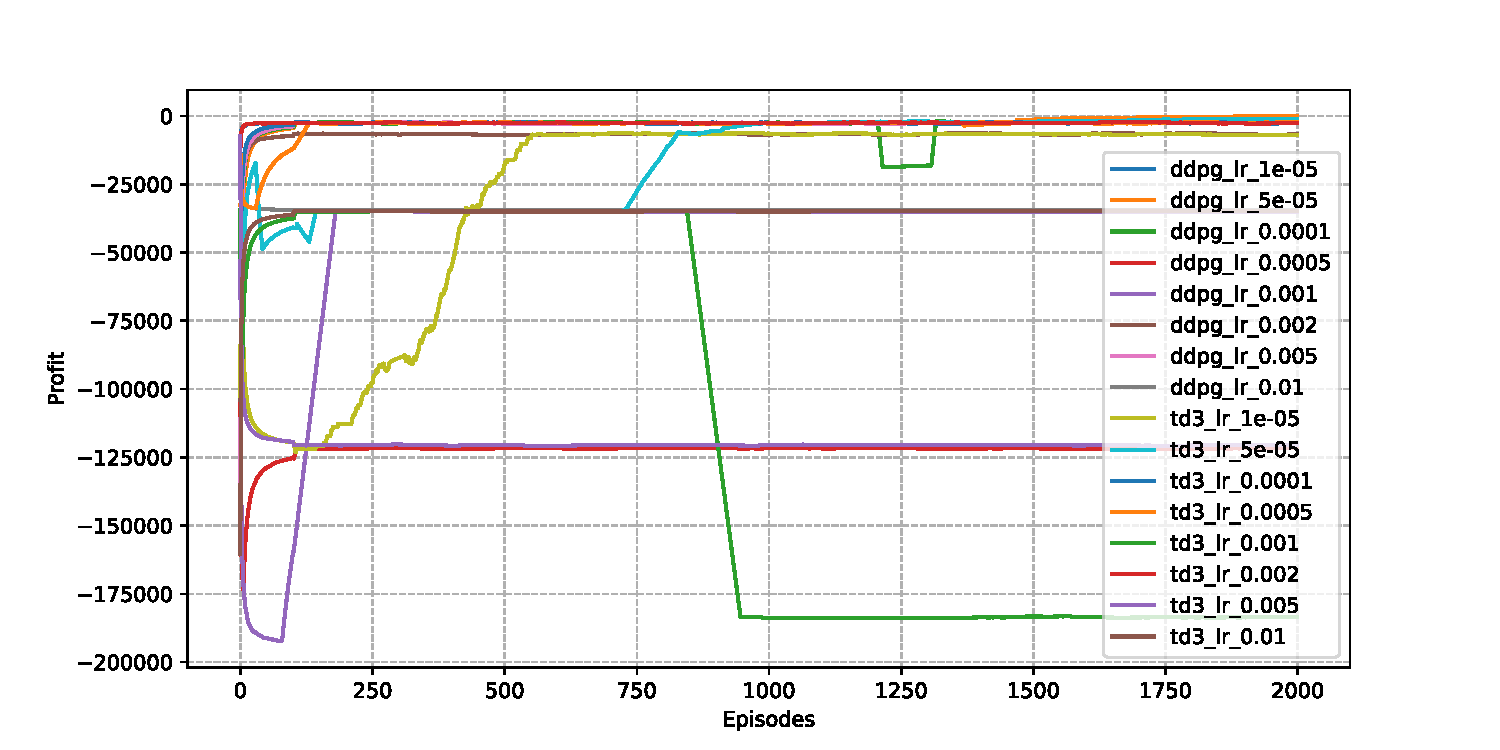
\includegraphics[width=\textwidth]{main/ddpg_td3.pdf}
	\caption{Lernkurven von DDPG und TD3 mit unterschiedlichen Lernraten}
	\label{graphic:DDPGLearningCurve}
\end{figure}

Die Lernkurven der beiden sehr ähnlichen Verfahren DDPG und TD3 sind in Abbildung \ref{graphic:DDPGLearningCurve} dargestellt.
Für jeden der beiden Algorithmen wurden acht Trainingsläufe durchgeführt, die mit unterschiedlichen Lernraten parametrisiert wurden.
Der Standardwert liegt für beide Algorithmen bei $10^{-3}$.
Es wurden Trainingsläufe mit diesen Lernraten sowie kleineren und größeren durchgeführt.
Die beim Training beobachteten Muster gleichen sich sowohl bei den beiden Algorithmen als auch den unterschiedlichen Parametrisierungen.
Zu Beginn des Trainings ist bei einigen Läufen eine Verbesserung der gemittelten Returns, die primäre Leistungskennziffer, zu beobachten.
Allerdings kommt diese Verbesserung bei allen Algorithmen zum Erliegen.
In keinem der Durchläufe konnten Gewinne erwirtschaftet werden.

Die schlechten Ergebnisse kommen deshalb zustande, weil die Agenten über das gesamte Training hinweg nicht lernen, sinnvolle Preise zu setzen.
Bei vielen Durchläufen bleiben die Neupreise ohne Anpassung auf die aktuelle Situation beim Maximum 10 hängen, oft sogar auch die Gebrauchtpreise.
Die Tatsache, dass die Agenten lange auf einer Stelle bleiben und auch die gleichen verbesserungswürdigen Aktionen immer wieder ausführen, könnte auf unzureichende Exploration schließen lassen.
Allerdings konnte auch eine verrauschte Aktionswahl zur besseren Exploration keine Verbesserung der Leistung bewirken.

Weiterhin sieht man in den Trainingsdurchläufen, dass sich die Leistung oft ruckartig verändert.
Der dabei in den Lernkurven zu erkennende lineare Auf- oder Abstieg ist der Durchschnittsbildung über die letzten hundert Episoden geschuldet.
Tatsächlich findet die Änderung sprunghaft statt.

Zahlreiche der Trainingsdurchläufe sind von starken Einbrüchen der Leistung geprägt.
Obwohl Instabilität bei DDPG und TD3 als Probleme bekannt sind, enttäuscht, dass trotz verschiedenster ausprobierter Werte in der Lernrate und Techniken zur verstärkten Exploration die Beherrschung dieses Marktes nicht erlernt werden konnte.
Deshalb werden in den folgenden Abschnitten DDPG und TD3 nicht weiter betrachtet.

\section{On-Policy-Learning -- A2C und PPO}
\label{section:main_ppo}
\begin{figure}[htb]
	\centering
	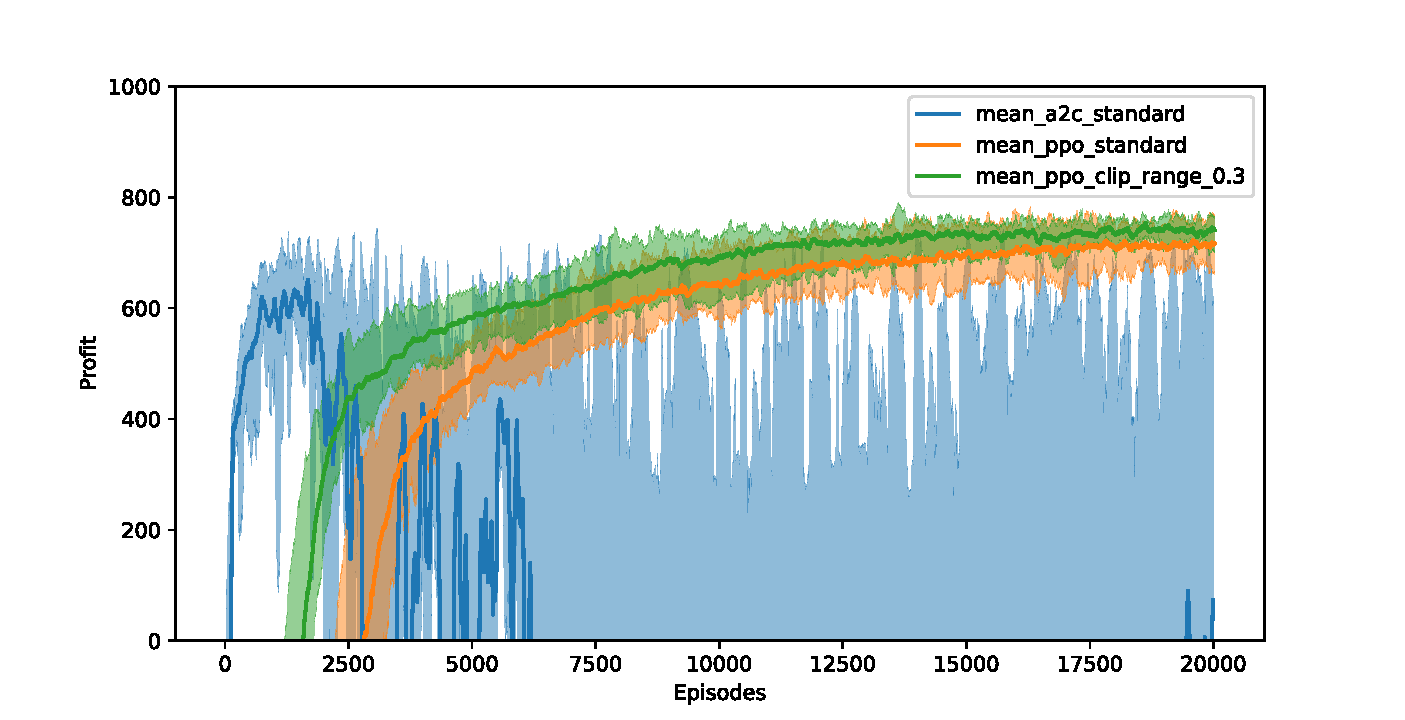
\includegraphics[width=\textwidth]{main/a2c_vs_ppo.pdf}
	\caption{Lernkurven von vier A2C- und vier PPO-Durchläufen auf dem Duopol mit unterbietendem Wettbewerber}
	\label{graphic:OnPolicyLearningCurves}
\end{figure}

Abbildung \ref{graphic:OnPolicyLearningCurves} stellt die Lernkurven der Algorithmen dar.
Dabei wurde PPO mit zwei Hyperparametrisierungen verwendet, die sich im Parameter $\epsilon$ unterscheiden.
Das eine Mal wird $0{,}2$ wie im Originalpaper verwendet, das andere Mal $0{,}3$.
Jedes dieser Experimente wurde vier Mal unabhängig für eine Million Schritte (zweitausend Episoden) durchgeführt.
Die Lernkurven verwenden wieder die laufenden Durchschnitte der Episodenreturns.
Der Bereich zwischen maximalem und minimalem Episodenreturns dieser vier Agenten ist eingefärbt.
Die Linie stellt ihren Durchschnitt dar.
In dieser Grafik wird der Verlustbereich ausgeblendet, um einen genaueren Vergleich im oberen Leistungsbereich zu ermöglichen.

Es fällt bei A2C ein sprunghafter Anstieg bei 100 Episoden auf.
Grund dafür ist der laufende Durchschnitt, bei dem nach 100 Episoden die sehr schlechten Ergebnisse vom Anfang des Trainings aus der Mittelung herausfallen.
Dieser Effekt tritt auch bei anderen Lernkurven-Diagrammen auf und liegt nur an diesem Diagrammtyp.

Aus der Grafik geht unmittelbar hervor, dass alle diese Agenten die Gewinnzone erreichen.
Sie erreichen alle mit Ergebnissen über 6000 pro Episode gute Ergebnisse.
Auf Grundlage dieser Grafik kann man feststellen, dass die Parametrisierung mit $\varepsilon=0{,}3$ bessere Performance einbringt als die Standardparametrisierung.

Für belastbare Aussagen über die Spitzenperformance wurde bei jedem Trainingsdurchlauf alle 100 Episoden das nach dem Rolling Average beste Modell aus den vorigen 100 Episoden gespeichert.
Nach dem Training wurden diese Modelle auf je 25 unabhängigen Episoden getestet, um eine genauere Schätzung ihrer Performance zu erhalten.
Die Leistungsmaxima der drei A2C-Trainingsdurchläufe lagen bei 8160, 8520, 7150 und 8510.
Bei den PPO-Durchläufen mit $\varepsilon=0{,}2$ waren die Maxima 7380, 7780, 8330 und 8120.
Die PPO-Durchläufe mit $\varepsilon=0{,}3$ erreichten 8300, 8680, 8360 und 8350.
Dass die Spitzen der A2C-Durchläufe in der Lernkurve niedriger sind als die hier aufgeführten Zahlen, liegt an den Rolling Averages und der erheblich geringeren Trainingsstabilität der A2C-Agenten.
Sie halten das hohe Leistungsniveau nur sehr kurz, weshalb die Mittelwertbildung mit anderen Ergebnissen während des Trainings niedrigere Werte ergibt.
Sichert man jedoch die Parameter der A2C-Agenten in dem Moment, in dem sie gerade gute Ergebnisse liefern, erzielen auch sie wettbewerbsfähige Leistung.

Die Advantage-Actor-Critic-Agenten erreichen das hohe Leistungsniveau nach deutlich weniger Episoden als die PPO-Agenten.
Ihr Durchschnitt überschreitet die Schwelle zum Gewinn nach etwa 60 Episoden.
\begin{figure}[htb]
	\centering
	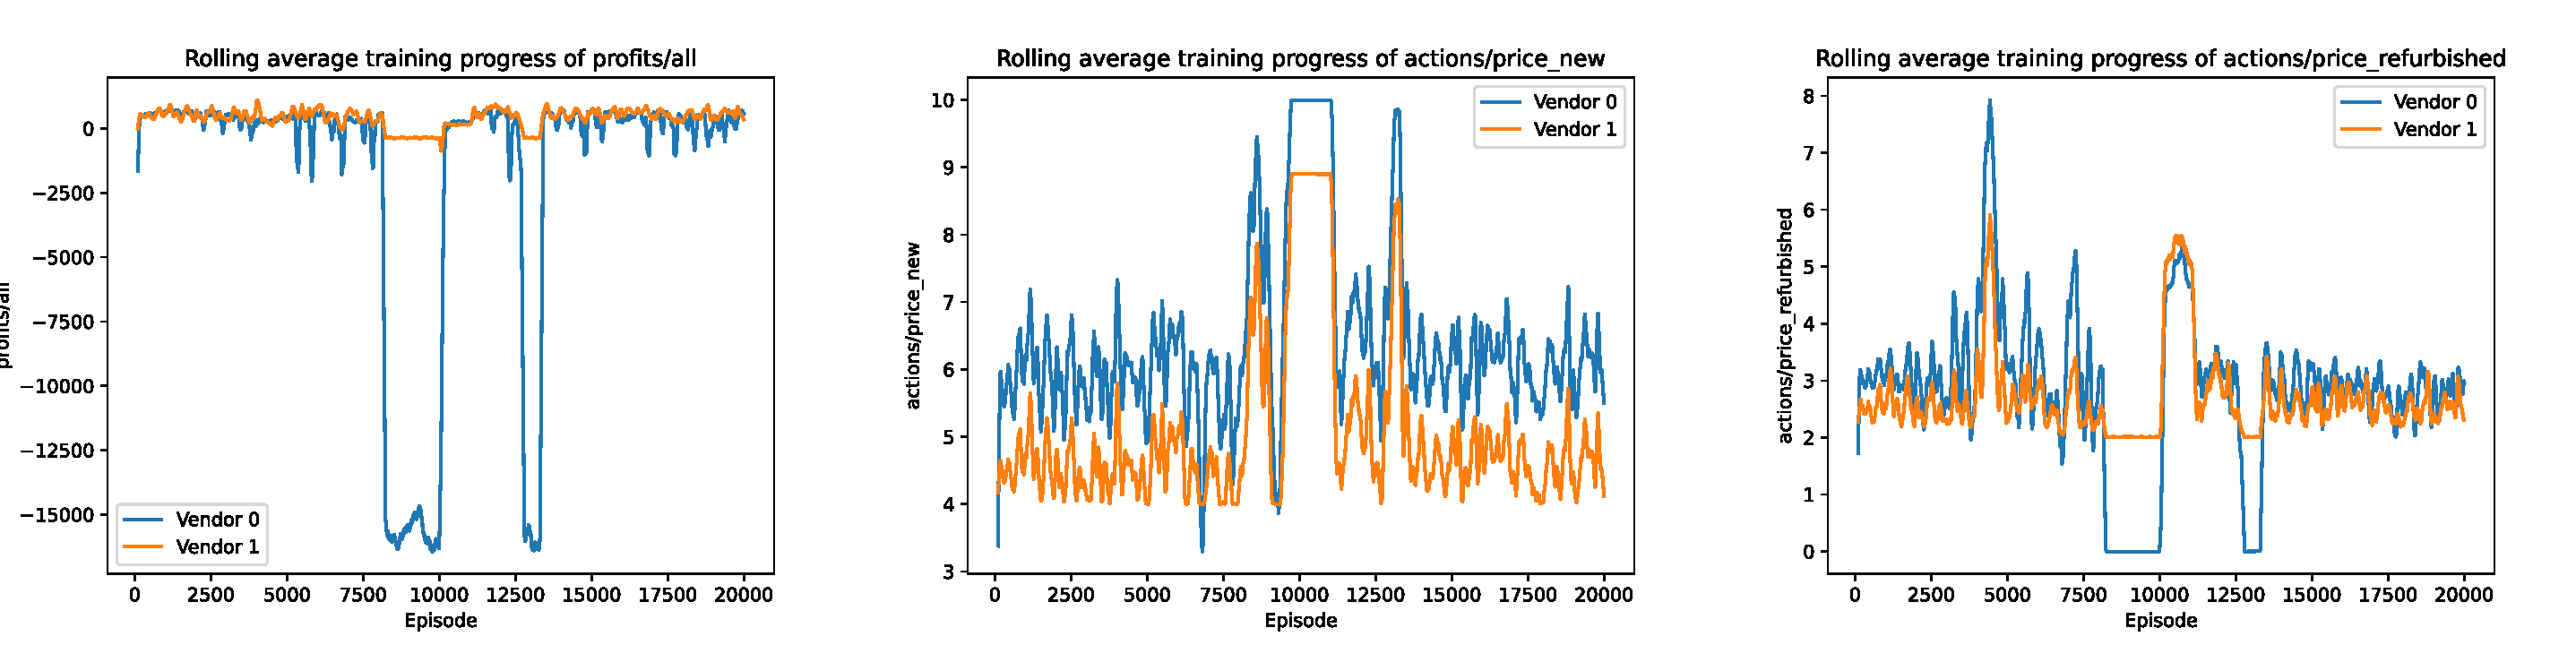
\includegraphics[width=\textwidth]{main/a2c_detailed_analysis.pdf}
	\caption{
		Detaillierte Betrachtung eines A2C-Trainingsdurchlaufes zur Visualisierung der Instabilität:
		(links) Lernkurve mit schnellem initialem Anstieg, danach Abstürze und Erholungen;
		(mittig) durchschnittliche Auswahl der Neupreise, zeigt erhebliche Schwankungen;
		(rechts) durchschnittliche Auswahl der Gebrauchtpreise, ebenfalls instabil
	}
	\label{graphic:A2CInstability}
\end{figure}
Die Grafik \ref{graphic:A2CInstability} stellt Details eines einzelnen A2C-Durchlaufes dar.
Es handelt sich dabei um einen typischen Durchlauf mit mittlerer Peak-Performance.
Man sieht die Instabilität nicht nur an den Ergebnissen, sondern auch an den starken Schwankungen, denen die Aktionsauswahl während des Trainings unterworfen ist.
Wie auch bei den anderen A2C-Agenten stürzt seine Leistung mitunter deutlich ab und fällt weit in die Verlustzone.
Nicht immer erholen sich die Agenten davon, oft erhalten sie weiterhin schlechte Ergebnisse.
Diese heftigen Abstürze führen dazu, dass die Mittelwertlinie der A2C-Agenten in Abbildung \ref{graphic:OnPolicyLearningCurves} wieder unter 0 fällt, obwohl einige der Agenten weiterhin akzeptable Ergebnisse liefern.

Im Gegenzug dazu ist die Trainingsstabilität bei den PPO-Varianten deutlich höher.
Zwischen den vier Trainingsdurchläufen der PPO-Agenten gibt es nur geringe Unterschiede.
Die Leistungsentwicklung liegt in einem schmalen Band und Abstürze finden nicht statt.
Allerdings benötigt PPO in der Standardkonfiguration knapp 250 Episoden und in der Version mit $\varepsilon=0{,}3$ ungefähr 180 Episoden, um die Gewinnzone zu erreichen.
Auch danach ist die Leistungssteigerung geringer als bei den anderen Algorithmen.
\begin{figure}[htb]
	\centering
	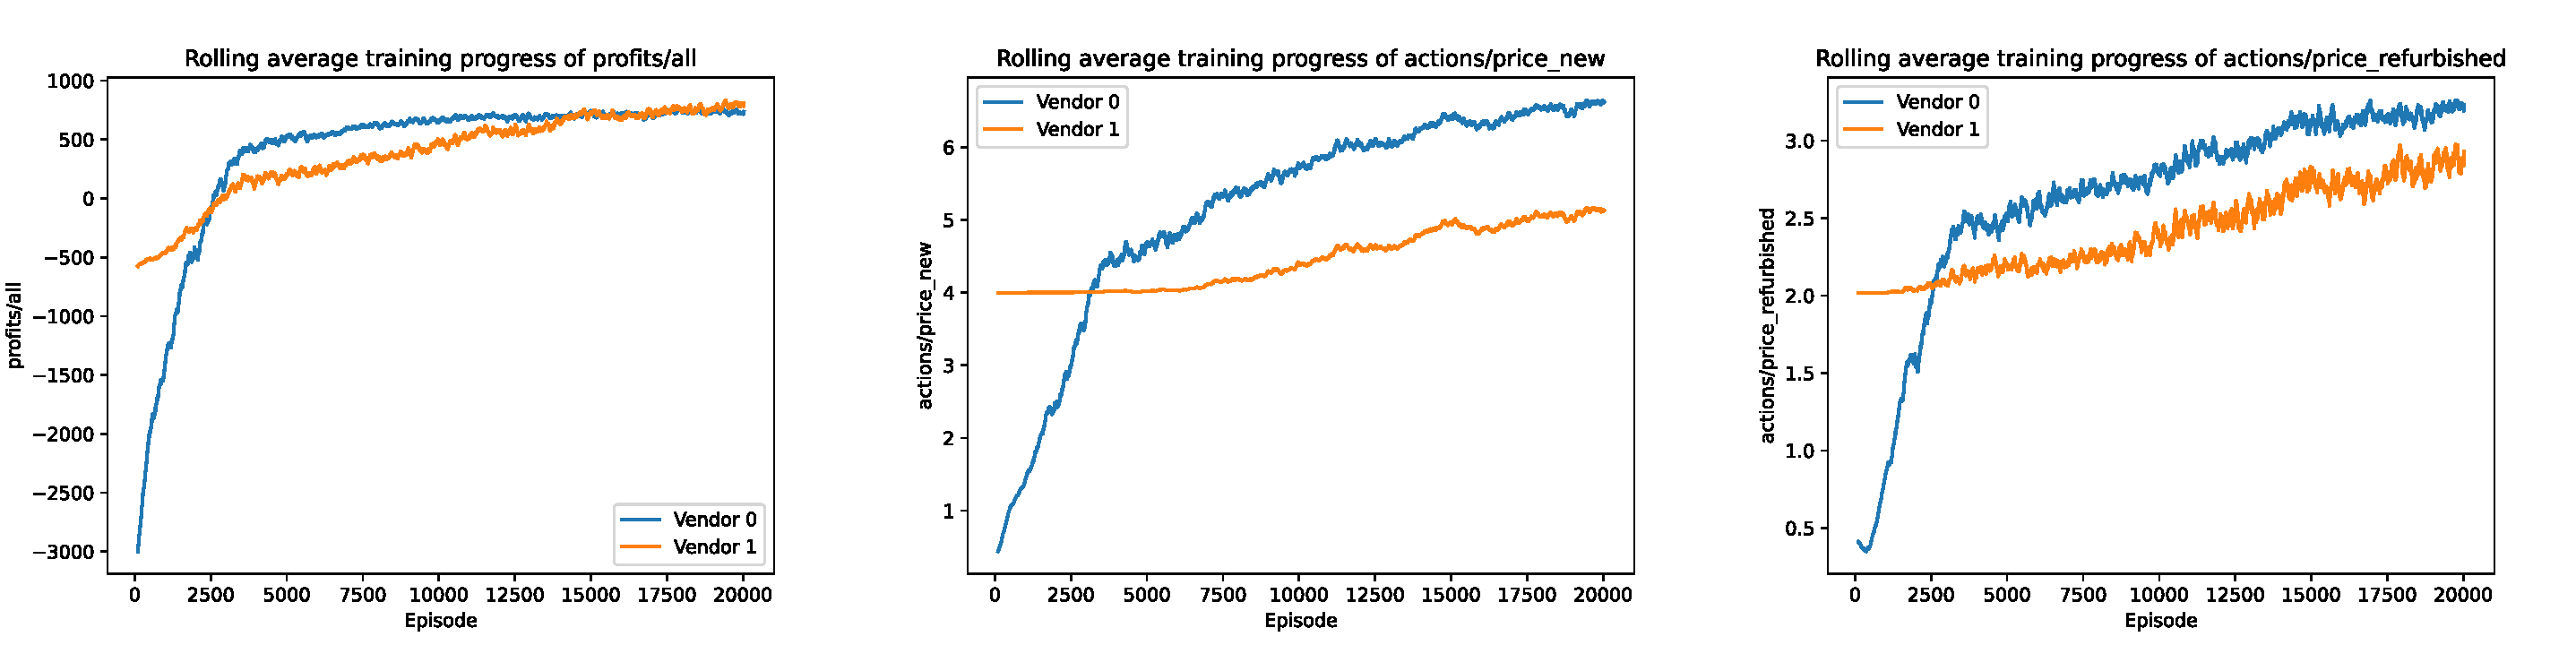
\includegraphics[width=\textwidth]{main/ppo_detailed_analysis.pdf}
	\caption{Detaillierte Betrachtung eines PPO-Trainingsdurchlaufes (Variante mit $\varepsilon=0{,}2$) analog zu Abbildung \ref{graphic:A2CInstability}}
	\label{graphic:PPOStability}
\end{figure}
In Abbildung \ref{graphic:PPOStability} ist ein detaillierter Blick in einen typischen PPO-Trainingsdurchlauf zu sehen.
Dessen durchschnittliche Performance steigt bis zum Ende auf 8160, und weist bei Return und der Aktionsauswahl eine durchweg stabile Entwicklung auf.

Der Unterschied in der Lerngeschwindigkeit und -stabilität zwischen PPO zu A2C überrascht nicht, er existiert \textit{by design}.
Diese Experimente zeigen, dass PPO in seiner Intention, die Trainingsstabilität zu erhöhen, erfolgreich ist.
Diese Erhöhung der Trainingsstabilität findet dadurch statt, dass die Änderung der stochastischen Policy bei den Trainingsschritten begrenzt wird.
Aus dieser Begrenzung der Policyänderung ist die geringere Lerngeschwindigkeit eine logische Schlussfolgerung.

So lässt sich auch erklären, warum der Durchlauf mit $\varepsilon=0{,}3$ schneller trainiert.
Mit größerem $\varepsilon$ wird pro Sample eine größere Policyänderung erlaubt, was zu schnellerem Training führt.
Allerdings steigt damit wieder das Risiko von Instabilität, weshalb die Parametrisierung des PPO-Algorithmus einen Trade-off zwischen Trainingsgeschwindigkeit und Stabilität eröffnet.
Die Wahl des Standardparameters $0{,}2$ mag in diesen Experimenten konservativ erscheinen, $0{,}3$ ist ebenfalls noch recht stabil, weist aber bereits kleinere Abstürze auf.
Das Experiment zu Abbildung \ref{graphic:PPODifferentClipping} im Anhang zeigt, wie sich PPO bei größerem $\varepsilon$ verhält.
Es bestätigt $0{,}3$ als eine gute Wahl.

Eine Beobachtung in Abbildung \ref{graphic:PPOStability} verdient besondere Beachtung, weil sie zunächst paradox erscheint:
Obwohl der RL-Agent den regelbasierten Agenten nach etwas Training übertrifft, wird er später wieder überholt.
Das erweckt den Eindruck, als würde der Agent im Verlaufe des Trainings schlechter.
Jedoch ist das Gegenteil der Fall.
Der PPO-Agent erlernt zunächst, die Preise für Neu- und Gebrauchtware höher zu setzen.
Dieses Training dauert aus den diskutierten Gründen im Vergleich lange, aber bei Neuverkaufspreisen, die größer als vier sind, macht er die Erfahrung, dass der regelbasierte Wettbewerber ihn immer um 1 unterbietet.
Durch wechselseitiges Unterbieten führt eine Preisabwärtsspirale dazu, dass sich der Preis nur knapp oberhalb des Einkaufspreises einpegelt.
Die dabei äußerst niedrige Rendite ermöglicht jedoch nur niedrige Gewinne, sodass der Agent in seinem weiteren Training die Erfahrung macht, dass er seinen Gewinn steigern kann, indem er seine Preise höher setzt.
Er wird dann weiterhin unterboten, allerdings nur um den Wert eins.
Dabei nimmt er in Kauf, dass mehr Kunden wegen des niedrigen Preises beim Konkurrenten kaufen und dieser bei steigenden Preisen auch an jedem Kunden mehr verdient.
Mit den Kunden, die der RL-Agent aber noch bekommt, kann er seine Gewinne im Vergleich zum niedrigpreisigen Markt dennoch steigern.
Der Effekt besteht also darin, dass der RL-Agent in Reaktion auf den ihn immer unterbietenden Konkurrenten diesem einen überproportionalen Gewinnanstieg erlaubt, um selbst mehr Gewinne machen zu können.
Die Existenz dieses Effekts ist der Tatsache geschuldet, dass das einzige Optimierungskriterium für die Agenten der eigene Gewinn ist.
Eine Rewardformulierung, die ein Übertreffen des Konkurrenten als Ziel mit einbezieht, wird in Abschnitt \ref{section:mixed_reward_function} behandelt.

\section{Soft Actor Critic}
\label{section:main_sac}
Auf dem gleichen Duopolmarkt wurde auch SAC ausprobiert.
Dabei wurde die SAC-Variante genommen, bei der der Entropiekoeffizient $\alpha$ automatisch trainiert wird.
Dieser hat sich bei allen Trainingsdurchläufen bei etwa $1,5$ eingependelt.
Die Grafik \ref{graphic:SACTemperature} im Anhang zeigt, dass unterschiedliche manuell eingestellte Entropiekoeffizienten ähnliche Trainingsergebnisse erreichen, wobei sich die Vermutung bestätigt, dass sehr niedrige Entropiekoeffizienten zu wenig Exploration bezwecken und Läufe mit deutlich höheren Entropiekoeffizienten wegen starker Regularisierung schlechtere Leistungsmaxima erreichen.

\begin{figure}[htb]
	\centering
	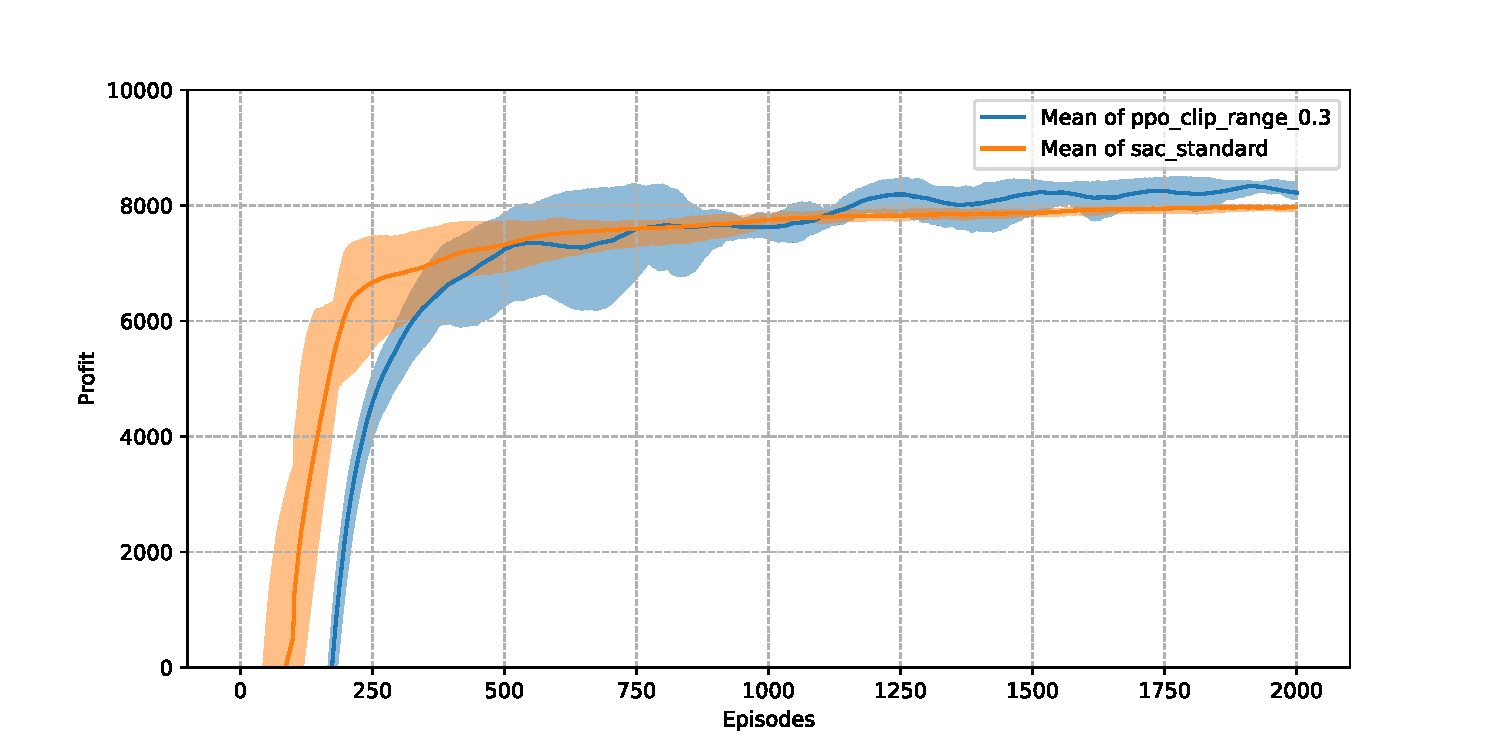
\includegraphics[width=\textwidth]{main/ppo_vs_sac.pdf}
	\caption{Lernkurven von vier SAC-Durchläufen im direkten Vergleich mit PPO}
	\label{graphic:SACLearningCurve}
\end{figure}

Grafik \ref{graphic:SACLearningCurve} zeigt die Lernkurve von vier Soft-Actor-Critic-Agenten bei einem Trainingsdurchlauf mit 2000 Episoden, genau so viele wie beim obigen Vergleich.
Zum Vergleich sind vier Trainingsdurchläufe mit PPO angegeben, die den aus Abschnitt \ref{section:main_ppo} bekannten Verlauf aufweisen.
Im Anhang in Abbildung \ref{graphic:SACvsA2CLearningCurve} ist die Lernkurve von SAC im direkten Vergleich mit A2C abgedruckt.

Soft-Actor-Critic wurde als Off-Policy-Algorithmus neben dem Erreichen von wettbewerbsfähigen Ergebnissen für zwei Hauptziele entwickelt:
Erstens soll es eine hohe Sample Efficiency haben, was bedeutet, dass es beim Training deutlich weniger Schritte benötigt.
Zweitens soll SAC eine hohe Trainingsstabilität haben.
Die Lernkurve bestätigt, dass Soft-Actor-Critic diese zwei Hauptziele erreicht.
Profitabel arbeitet der Agent nach etwa 70 Episoden, was nur leicht hinter A2C liegt und erheblich besser als PPO ist.
Ab etwa 250 bis 300 Episoden sind die Agenten nah an ihrer Peak-Performance.
Das restliche Training bringt nur noch kleine Leistungszugewinne.
Die hohe Sample-Efficiency liegt daran, dass SAC die gesammelte Erfahrung im Experiencebuffer speichert und sehr oft zum Training nutzt.
Dadurch werden viel weniger Samples als bei PPO benötigt, das alte Erfahrung nicht mehr verwenden kann, sobald sich die Policy geändert hat.
Alle vier Agenten bewegen sich für den Rest des Trainings in einem schmalen Bereich, wobei der Durchschnittsreturn knapp 8000 erreicht.
Ob weiteres Training zusätzliche Verbesserungen bezwecken können, lässt sich nicht sicher sagen.
Allerdings ändern sich die gemessenen Kenngrößen wie Aktionsauswahl und Loss im späteren Verlauf des Trainings kaum noch.
Der Durchschnitt der vier SAC-Agenten liegt zwar dauerhaft über dem Durchschnitt der A2C-Agenten, aber gute A2C-Durchläufe erreichen bessere Performance in der Spitze als die SAC-Agenten.
Die Maximalleistungen dieser vier SAC-Durchläufe liegen bei 8120, 7890, 8120 und 8160.
Damit bleiben sie ebenfalls hinter denen der PPO-Agenten zurück, die meist über 8300 als Return erzielen.

\begin{figure}[htb]
	\centering
	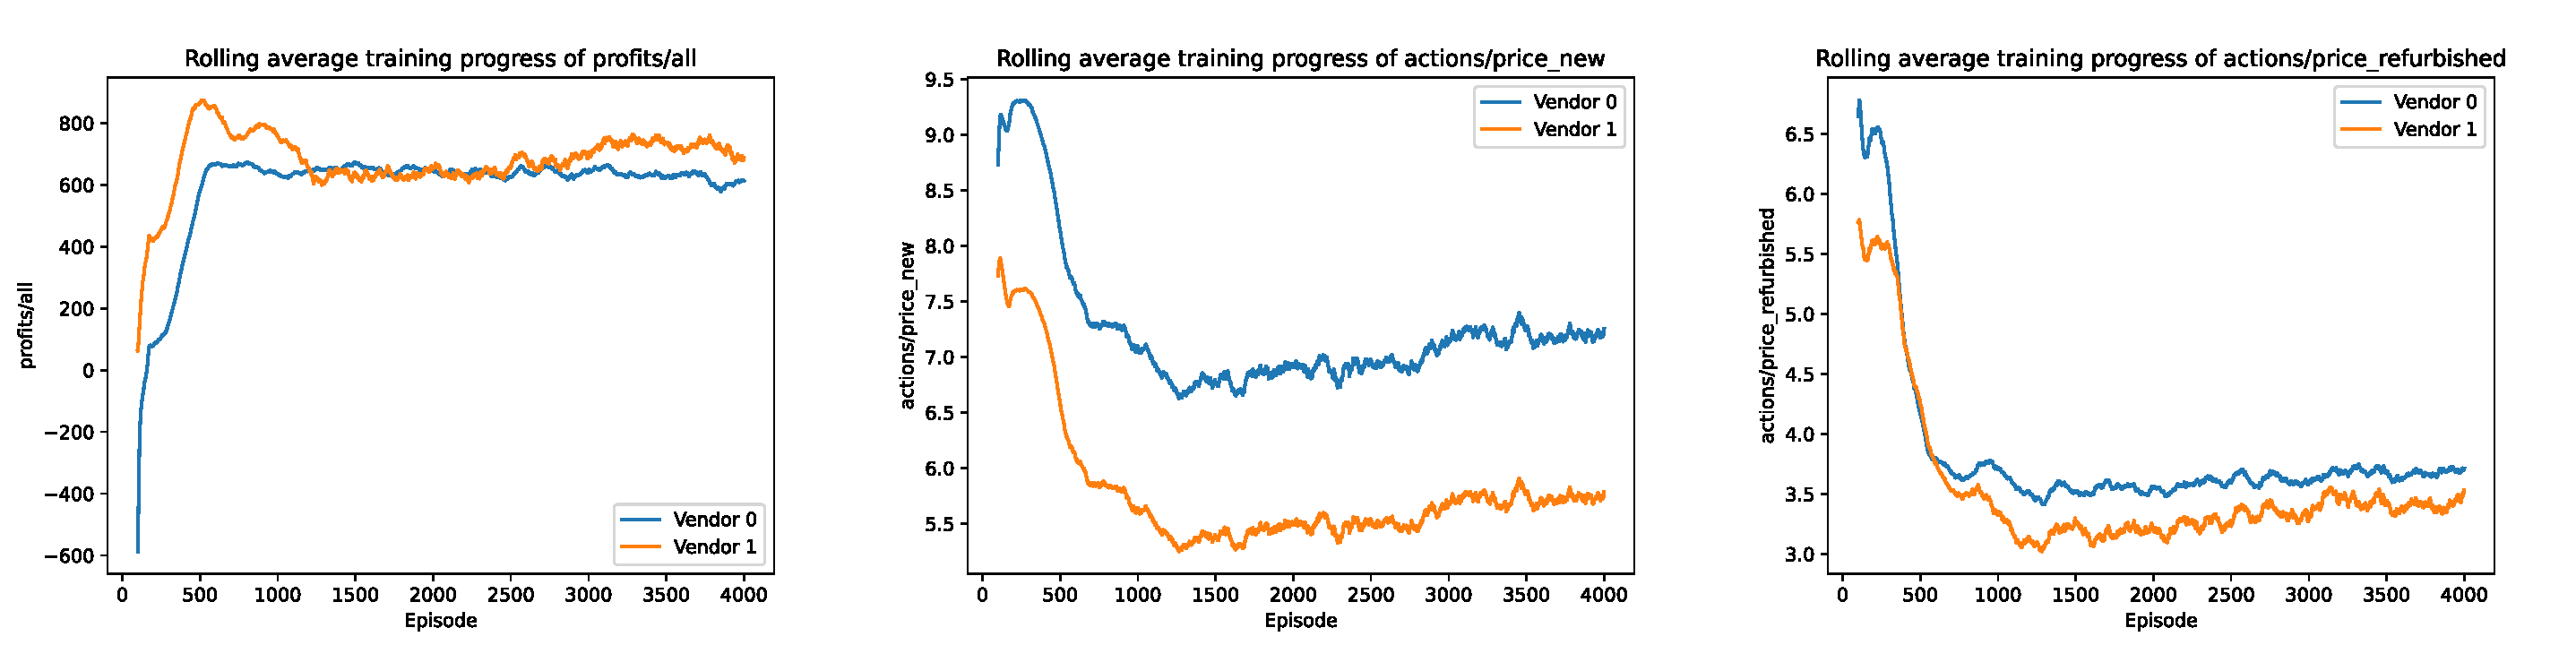
\includegraphics[width=\textwidth]{main/sac_detailed_analysis.pdf}
	\caption{Detaillierte Betrachtung eines SAC-Trainingsdurchlaufes}
	\label{graphic:SACDetails}
\end{figure}

Wie auch für die anderen Algorithmen wurden für SAC ein typischer Durchlauf und die gemittelten Aktionen in Abbildung \ref{graphic:SACDetails} abgedruckt.
Die durchschnittlichen Preise starten -- offenbar durch eine andere Parameterinitialisierung -- auf höherem Niveau als bei PPO.
Sie sinken dann und enden bei $6{,}4$ und $5{,}4$, genau wie bei PPO.

Warum PPO in diesem Markt etwas besser abschneidet, ist eine äußerst interessante Frage, deren Beantwortung man sich aber auf Grundlage dieser Experimente nur annähern kann.
Eine plausible Erklärung wird in Abschnitt \ref{section:partial_markov} auf Grundlage der dortigen Beobachtungen geliefert.
Kurz ausgedrückt wird dort festgestellt, dass SAC in der Policy Zusammenhänge lernt, die nicht gelernt werden sollten.
Eine andere mögliche Erklärung, dass die Policy der SAC-Agenten wegen der Entropieregularisierung größere Standardabweichungen schätzt und deshalb weniger genau als die von PPO ist, lässt sich durch die Daten aus dem Training nicht bestätigen.
Bei beiden Trainingsalgorithmen haben die Policies zum Ende des Trainings Standardabweichungen von etwa $0{,}5$, wobei SAC keine größeren Standardabweichungen hat.

Für die Frage >>Wie lange dauert das Training?<< gibt es zwei mögliche Kenngrößen.
Einmal kann die Anzahl der benötigten Samples bewertet werden, die Sample Efficiency, oder es kann die tatsächliche Zeit auf der Uhr herangezogen werden.
Letztere hängt stark von der Hardware sowie der Geschwindigkeit der Simulation im Vergleich zum Optimieren der Parameter ab.
Bei der für diese Experimente verwendeten Implementierung und Hardware benötigt das Training pro Schritt mit SAC etwa $3{,}7$ Mal so lang wie mit PPO.
Das Sammeln der Beispiele aus dem Markt nimmt bei PPO etwa 25\% der Trainingszeit ein, bei SAC nur etwa 6\%.
Die Geschwindigkeit des Trainings ist bei A2C und PPO sehr ähnlich.
Rechnet man somit die tatsächliche Trainingszeit, relativiert sich der höhere Samplebedarf bei PPO.
Insbesondere wird deutlich, dass A2C in reinem Zeitbedarf den anderen Algorithmen erheblich überlegen ist.

Weil insbesondere das SAC-Training so zeitaufwändig ist und der Lernfortschritt im späteren Verlauf so gering ist, wird bei einigen der folgenden Versuche mit SAC die Anzahl der Trainingsschritte reduziert.
Gleiches geschieht bei A2C, da hier bereits sehr früh die maximale Performance erreicht werden.

\section{Den Konkurrenten übertreffen -- eine angepasste Rewardfunktion}
\label{section:mixed_reward_function}
In den bisher untersuchten Lernkurven erreichen die Agenten zwar sehr gute Profite, lassen sich aber vom regelbasierten Konkurrenten übertreffen.
In Abschnitt \ref{section:main_ppo} wurde bereits erklärt, dass dies nicht als Schwäche der Algorithmen zu deuten ist, sondern auf die Rewardfunktion zurückgeführt werden kann, die nur eigenen Profit bewertet.
Nun ist die Maximierung des eigenen Profits keine ungeeignete Kenngröße, dennoch werden Unternehmen ungern ihren Konkurrenten in einem symmetrischen Markt mehr Gewinn überlassen als sich selbst.
Deshalb liegt es nahe, in der Belohnungsfunktion nicht nur die eigenen Profite zu bewerten, sondern auch, ob der Konkurrent übertroffen wird.

Eine Möglichkeit besteht darin, den Markt als \textit{Zero-Sum-Spiel} zu formulieren, indem die Belohnung genau die Differenz aus eigenem Gewinn und dem des Konkurrenten ist.
Diese Formulierung legt den klaren Fokus auf das Übertreffen des Konkurrenten und eröffnet weiterhin möglicherweise das Marktszenario für Erkenntnisse aus der Spieltheorie für Zero-Sum-Spiele.
Allerdings ist diese Formulierung nicht praxistauglich, weil das Ziel der Profitmaximierung gar nicht bewertet wird.
So kann es passieren, dass bei einer Optimierung der Differenz zwar der Konkurrent deutlich übertroffen wird, allerdings bei insgesamt niedrigen Gewinnen oder sogar in der Verlustzone.

Deshalb wurde für die folgende Versuchsreihe eine gemischte Rewardfunktion verwendet.
Sie berechnet einfach die Summe aus Profit und Differenz zum Konkurrenten.
Für diese Experimente wurden beide Summanden gleich gewichtet, es könnte aber ein Hyperparameter eingefügt werden, um die beiden Ziele Profitmaximierung und Übertreffen des Konkurrenten zu balancieren.

\begin{figure}[htb]
	\centering
	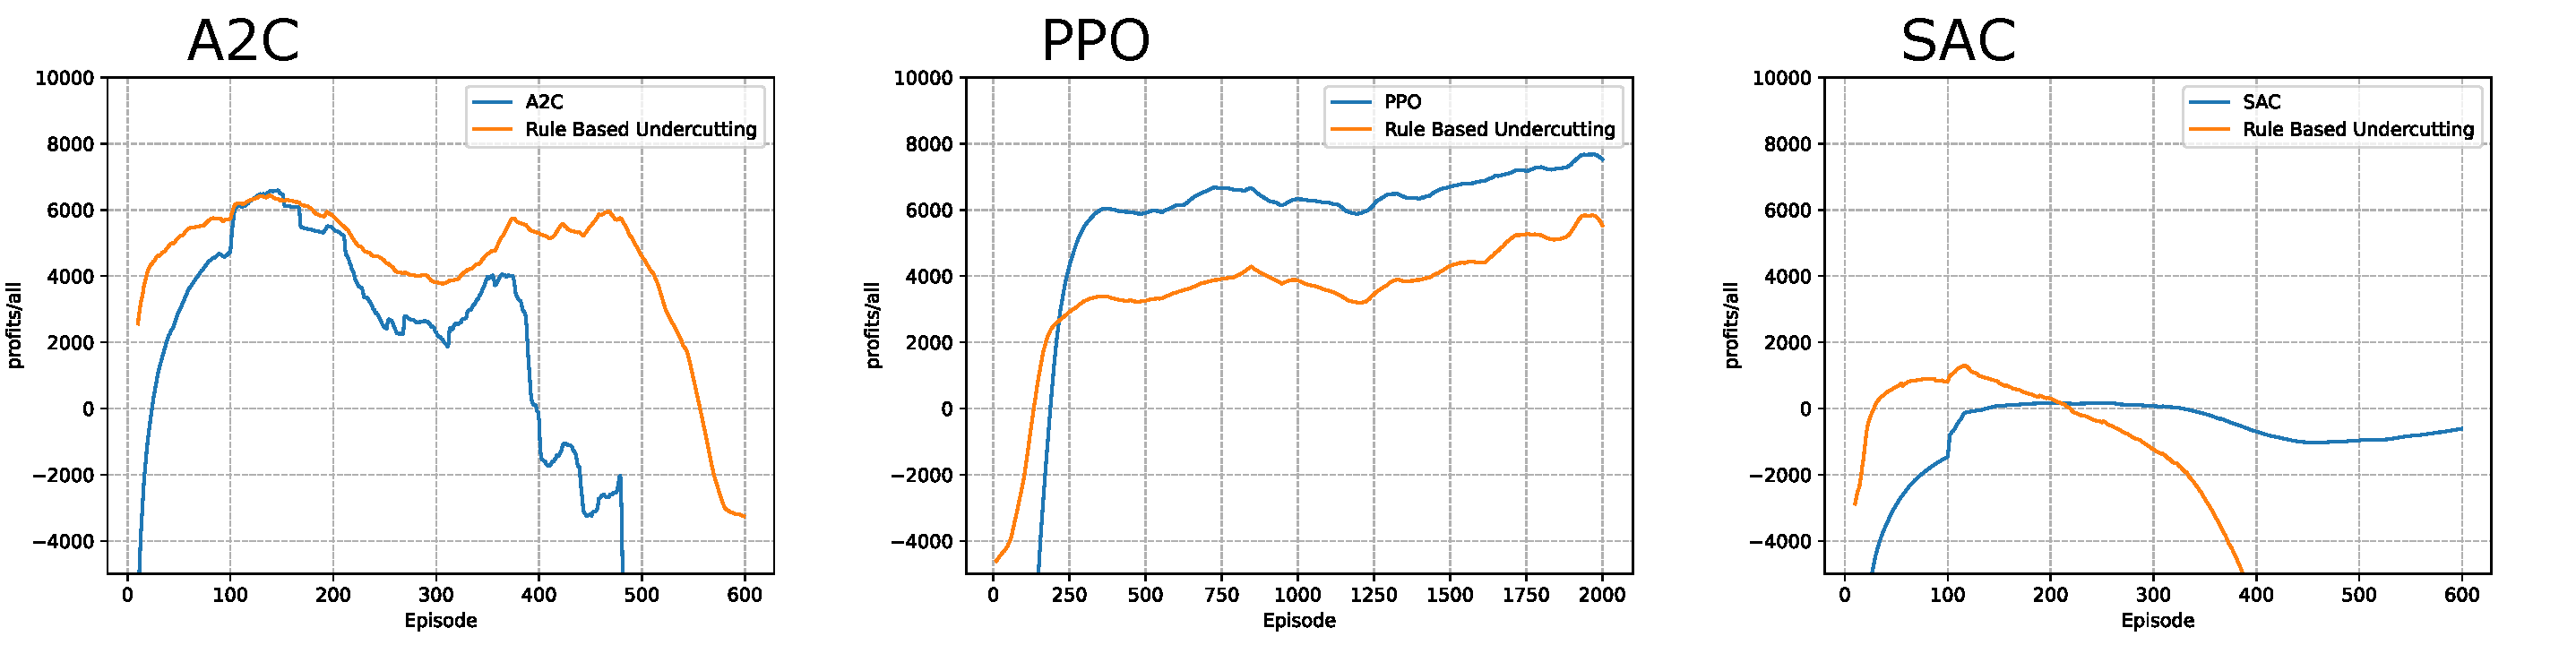
\includegraphics[width=\textwidth]{main/lineplot_mixed_rewards.pdf}
	\caption{Repräsentative Durchläufe der Algorithmen bei gemischter Rewardfunktion}
	\label{graphic:LineplotMixedRewards}
\end{figure}

Im Anhang sind die Lernkurven der Algorithmen mit gemischter Rewardfunktion im Vergleich zur Standardrewardfunktion abgedruckt (Abbildungen \ref{graphic:MixedRewardsA2C}, \ref{graphic:MixedRewardsPPO} und \ref{graphic:MixedRewardsSAC}).
Wie erwartet liegen die Gewinne der Agenten niedriger als bei der anderen Rewardfunktion (schließlich sind Gewinne nicht mehr das alleinige Optimierungskriterium), allerdings fällt dieser Unterschied bei den Algorithmen unterschiedlich aus.
Weiterhin erhöht sich durch den Wechsel der Rewardfunktion die Instabilität bei allen Algorithmen.
Ob das Ziel, neben guten Gewinnen die Konkurrenz zu überholen, erreicht wird, zeigt \mbox{Abbildung \ref{graphic:LineplotMixedRewards}}.

Obwohl der A2C-Durchlauf wieder Probleme mit Instabilität zeigt, erreicht er ein durchschnittliches Maximum von 7900, der Konkurrent nur 7200.
Er überholt also bei der veränderten Rewardfunktion den regelbasierten Konkurrenten, und erhält gleichzeitig gute Gewinne.

Beim PPO-Durchlauf ist genau das zu sehen, was Ziel der Anpassung der Rewardfunktion war:
Der PPO-Agent bleibt nach dem ersten Übertreffen des Konkurrenten diesem über das gesamte Training hinweg voraus und erreicht ein Maximum von 8000 im Vergleich zu 6100 des regelbasierten Konkurrenten.

Der Soft-Actor-Critic-Durchlauf erreicht nach der gemischten Rewardfunktion sogar die besten Ergebnisse, obwohl der Agent selbst in die Verlustzone rutscht.
Er hat eine Policy gefunden, bei der der regelbasierte Konkurrent ständig Strafen zahlen muss, weil er keine gebrauchten Produkte liefern kann.
Dadurch macht der regelbasierte Konkurrent einen deutlich größeren Verlust
Die Details zu diesem Durchlauf sind interessant und in Abbildung \ref{graphic:ExplanationUnnormalSAC} im Anhang erläutert.
Aus Sicht der Algorithmenanalyse ist es ein bemerkenswertes Resultat, dass der SAC-Agent dazu fähig war, eine solche Strategie zu explorieren und zu entwickeln.
Für die praktische Verwendung ist diese Policy allerdings nicht geeignet.
Der Profit des Agenten sollte beim Design der Rewardfunktion höher gewichtet werden.

\section{Training gegen die eigene Policy}
\label{section:self_play}
In den Durchläufen aus den Abschnitten \ref{section:main_ddpg}, \ref{section:main_ppo} und \ref{section:main_sac} trainierten die RL-Agenten alle gegen den unterbietenden, regelbasierten Wettbewerber.
Das erfüllt die theoretischen Anforderungen eines Markov-Entscheidungsprozesses, wirft jedoch für praktische Anwendungen eine Reihe von Problemen auf.
Erstens muss dafür die Policy des Konkurrenten bekannt sein.
Weil jedoch davon ausgegangen werden kann, dass der Konkurrent seine Preisstrategie nicht verraten wird, müsste sie unter Inkaufnahme von Ungenauigkeiten aus historischen Daten geschätzt werden.
Zweitens ist die mittels RL trainierte Strategie nur gegen diese bestimmte regelbasierte Strategie gerichtet.
Ändert der Wettbewerber seine Preisstrategie plötzlich, schwächt das die Performance der RL-Strategie und macht neues Training erforderlich.

Deshalb wünscht man sich eine Strategie, die gegen möglichst viele Wettbewerberstrategien bestehen kann, und nicht auf eine spezielle überangepasst ist.
DeepMind hatte eine ähnliche Herausforderung beim Training von Go- und Schachstrategien, das durch Self-Play gelöst wurde. 
Das kann in \cite{Silver2017, https://doi.org/10.48550/arxiv.1712.01815} nachgelesen werden.

Für diesen Markt wurde eine Self-Play Variante entwickelt, bei der ein RL-Agent weiterhin auf einem Duopol-Markt trainiert, aber die Policy des Wettbewerbers die eigene Policy ist.
In der programmiertechnischen Umsetzung wird für den Gegner ein Zeiger auf den RL-Agenten übergeben, der schließlich auch die Policyfunktion implementiert.
Dadurch, dass der Agent stets gegen sich selbst spielt, wird die Markov-Eigenschaft verletzt, dennoch zeigen die Ergebnisse Trainingserfolg.
Die Motivation hinter Self-Play ist, dass der Agent einerseits die ganze Zeit einem ebenbürtigen Gegner gegenübersteht, aber andererseits auch, dass er ständig Strategien gegen die eigene entwickelt, die dann wiederum herausgefordert werden.
Dadurch soll der Agent auf eine Vielzahl von Policies vorbereitet werden.

Experimente mit Self-Play wurden mit den Algorithmen durchgeführt, die sich in der vorangegangenen Analyse als grundsätzlich geeignet für diesen Markt erwiesen haben: A2C, PPO und SAC.
Dabei wurde die gesamte Versuchsreihe mit der normalen Rewardfunktion und der gemischten Rewardfunktion aus Abschnitt \ref{section:mixed_reward_function} durchgeführt.

\begin{figure}[htb]
	\centering
	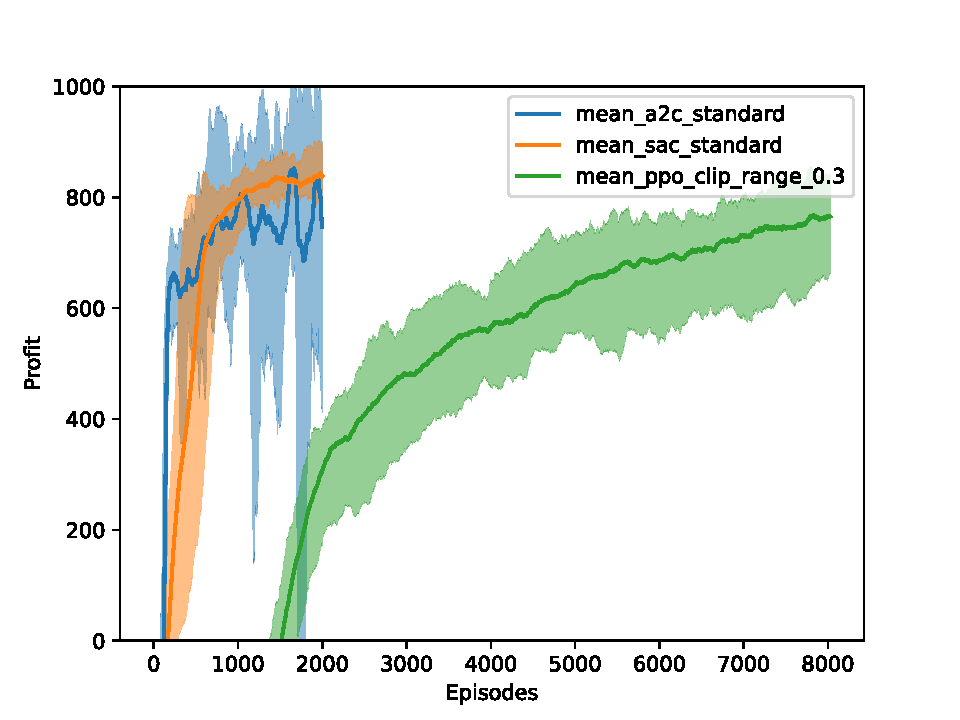
\includegraphics[width=\textwidth]{main/self_play.pdf}
	\caption{Lernkurve von vier A2C-, PPO- und SAC-Durchläufen beim Self-Play; die Algorithmen wurden über 2000 Episoden trainiert}
	\label{graphic:SelfPlayLearningCurve}
\end{figure}
In der Abbildung \ref{graphic:SelfPlayLearningCurve} sind die Lernkurven der drei Algorithmen beim Training gegen sich selbst abgedruckt.
Die Lernkurven bei gemischter Rewardfunktion sehen ähnlich aus und sind im Anhang in Abbildung \ref{graphic:SelfPlayMixedLearningCurve} zu finden.
Diese Kurven zeigen zunächst, dass Lernerfolg bei allen dieser drei Agenten erreicht wird.
Sie alleine können allerdings nicht aussagen, ob die Agenten sich tatsächlich gegen die Konkurrenz behaupten können.
Deshalb dürfen auch die Returns dieser Lernkurven nicht mit denen aus den vorigen Abschnitten verglichen werden.

\begin{figure}[htb]
	\centering
	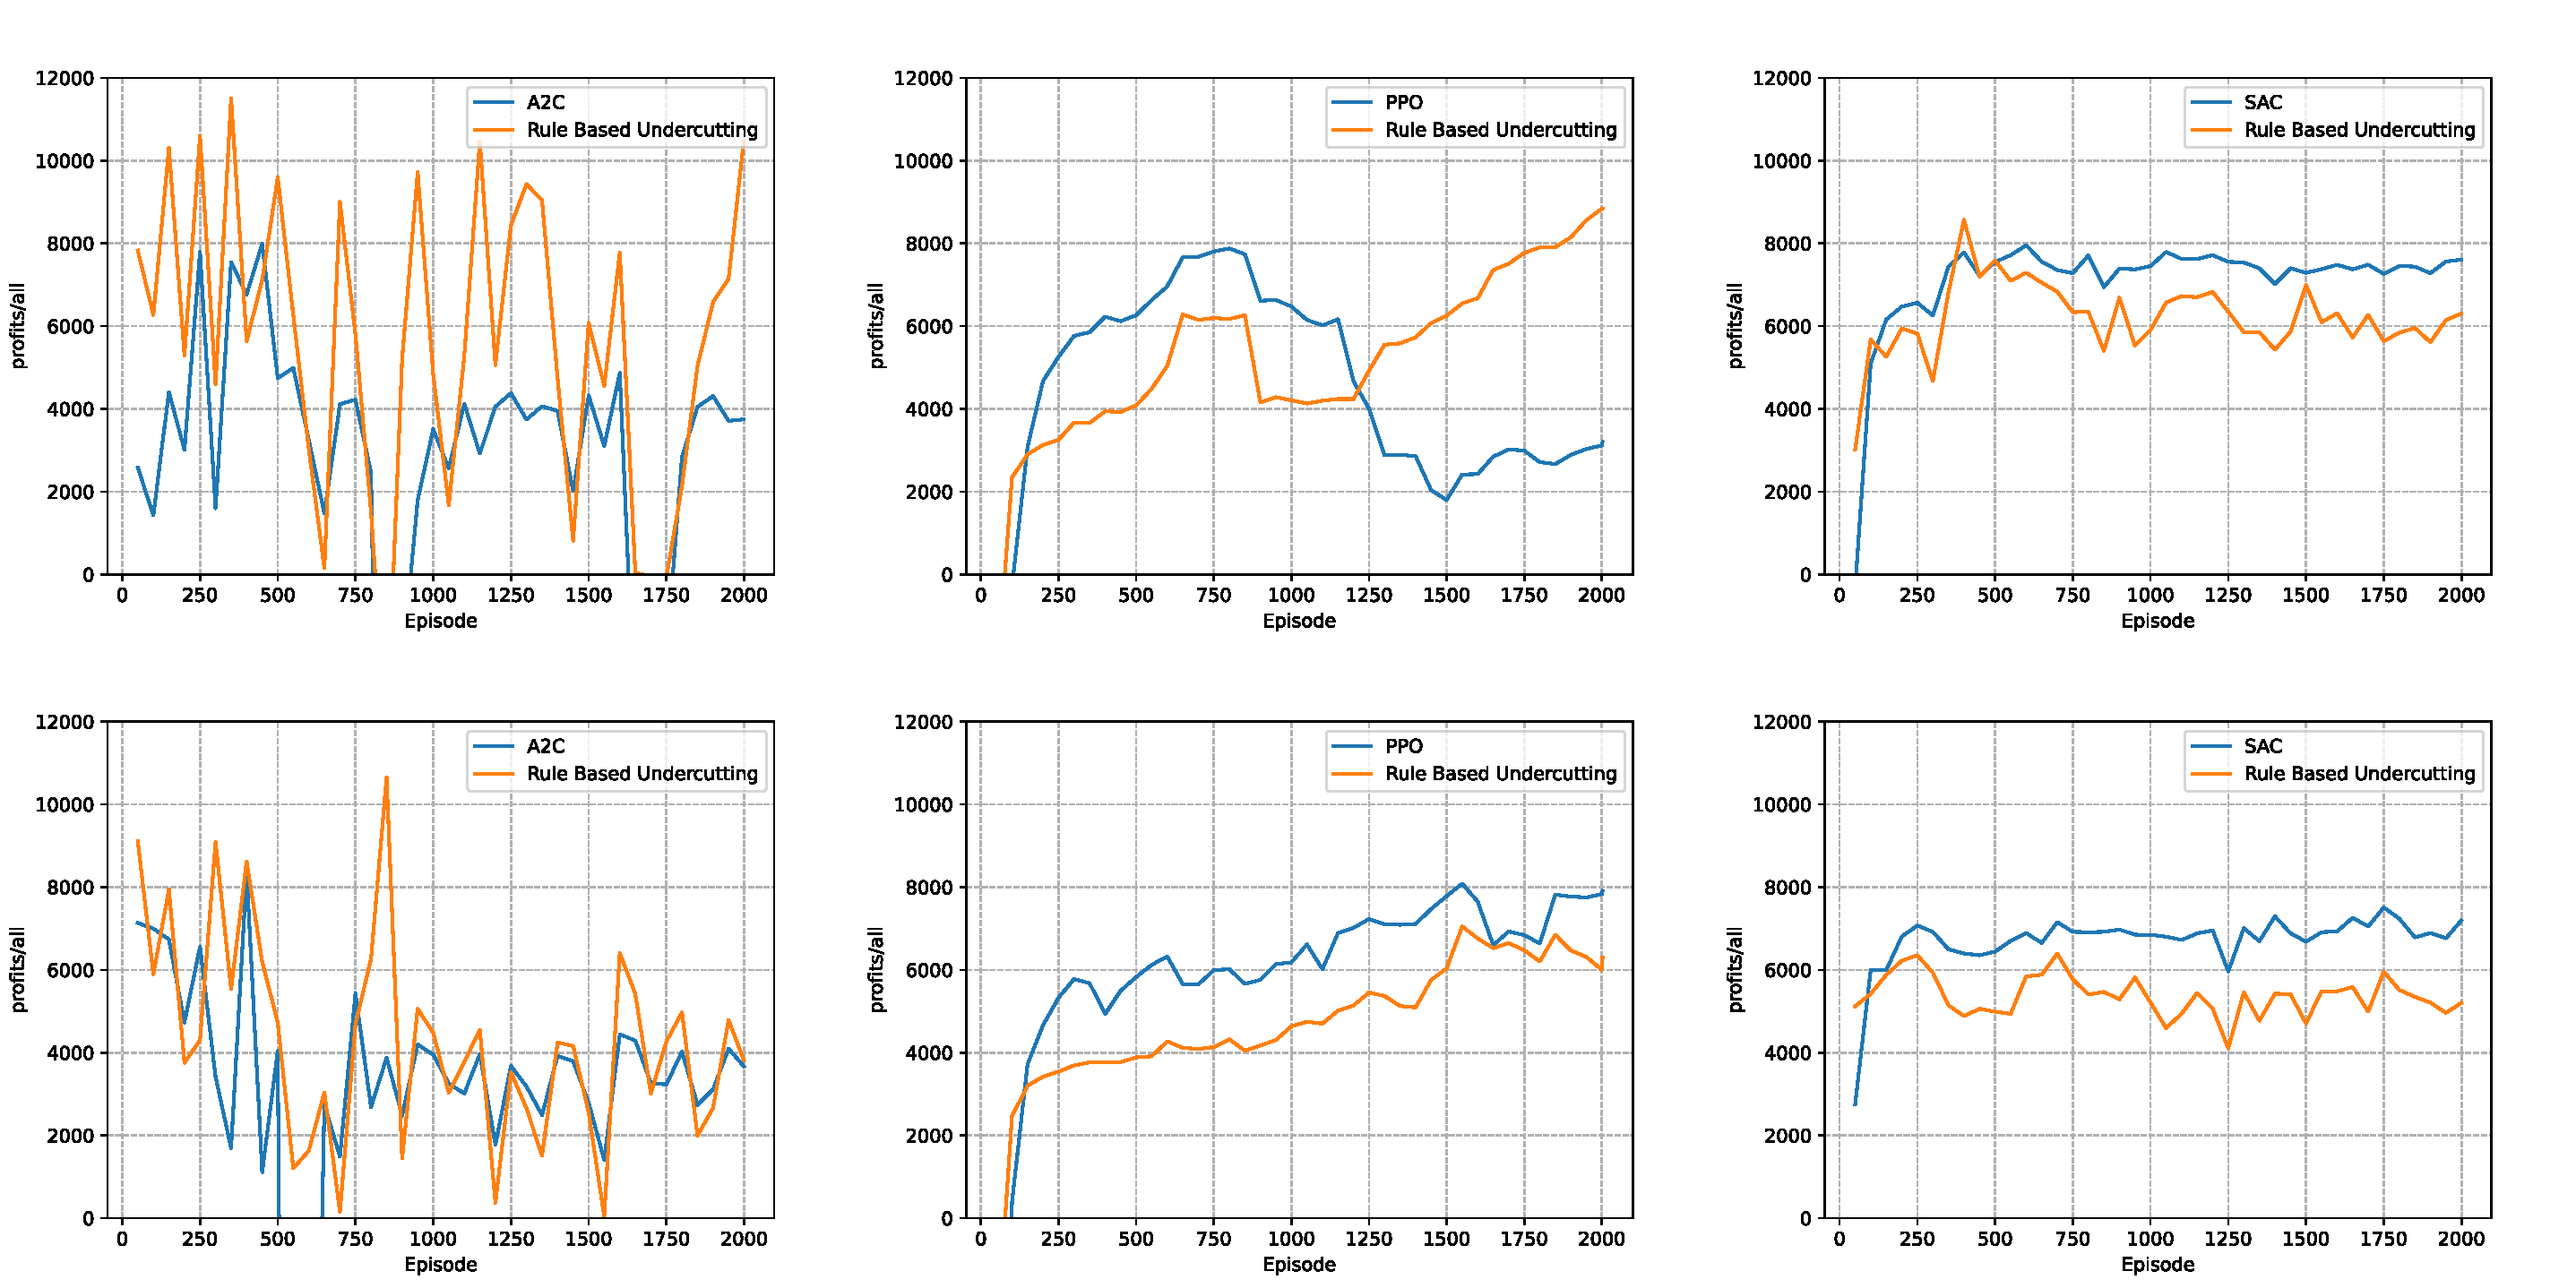
\includegraphics[width=\textwidth]{main/self_play_detailed.pdf}
	\caption{Repräsentative Self-Play Durchläufe; spaltenweise nach Agenten: (links) A2C, (mittig) PPO, (rechts) SAC; obere Zeile mit normaler Rewardfunktion, untere Zeile mit gemischter Rewardfunktion}
	\label{graphic:SelfPlayDetails}
\end{figure}
Um Vergleichbarkeit herstellen zu können, wurde während des Self-Plays alle 50 Episoden ein Modell gespeichert und jedes dieser Modelle anschließend für 25 Episoden getestet.
Damit wurden akkurate Lernkurven erstellt, die das beim Self-Play trainierte Modell mit dem regelbasierten Agenten vergleichen.
Für die drei Algorithmen und die zwei Rewardfunktionen wurde ein mittlerer Durchlauf ausgewählt und in der \mbox{Abbildung \ref{graphic:SelfPlayDetails}} veranschaulicht.

Bei beiden Rewardfunktionen haben die Agenten den Markt erfolgreich erlernt und können sich auch in dem Benchmark gegen den regelbasierten Konkurrenten behaupten.
So liegen die Peaks aller Agenten im Benchmark bei 8000 oder knapp darunter, allerdings mit starken Schwankungen bei A2C.
Von den A2C-Agenten erreichen einige kein Niveau von 5000.
Die Auswirkungen der gemischten Rewardfunktion sind bei den Trainingsdurchläufen zu erkennen.
Dass während des Trainings die Differenz zwischen eigenem und gegnerischem Profit mit als Optimierungskriterium verfolgt wird, führt tatsächlich dazu, dass der durch Self-Play trainierte Agent auch im Vergleich mit dem regelbasierten Konkurrenten sich zumindest nicht übertreffen lässt (A2C), den Konkurrenten im Gegensatz zur normalen Rewardfunktion dauerhaft abhängt (PPO) oder den Abstand zum Konkurrenten vergrößert (SAC).

Obwohl die Benchmarkergebnisse erwartungsgemäß nicht ganz an die Ergebnisse des Trainings direkt gegen den regelbasierten Agenten heranreichen, so sind sie nahe daran.
Das ist bemerkenswert, da diese Erfolge im Benchmark erreicht wurden, ohne den regelbasierten Wettbewerber je vorher gesehen zu haben.
Damit können diese Experimente als erfolgreich gewertet werden.
Die Fähigkeiten vom Training gegen die eigene Policy werden damit auch für ein Duopol bestätigt.

\section{Partielle Beobachtungen}
\label{section:partial_markov}
Für die Markov-Eigenschaft ist ein sechsdimensionaler Aktionsraum erforderlich.
Jedoch ist die Beobachtung mancher der verwendeten Größen in der Praxis nicht machbar.
So wird der Konkurrent sich nicht ins Lager schauen lassen, und die Anzahl der Produkte in Zirkulation ist schwer zu schätzen.
Deshalb drängt sich die Frage auf, ob die Algorithmen auch ohne diese beiden Informationen funktionieren.

\begin{figure}[htb]
	\centering
	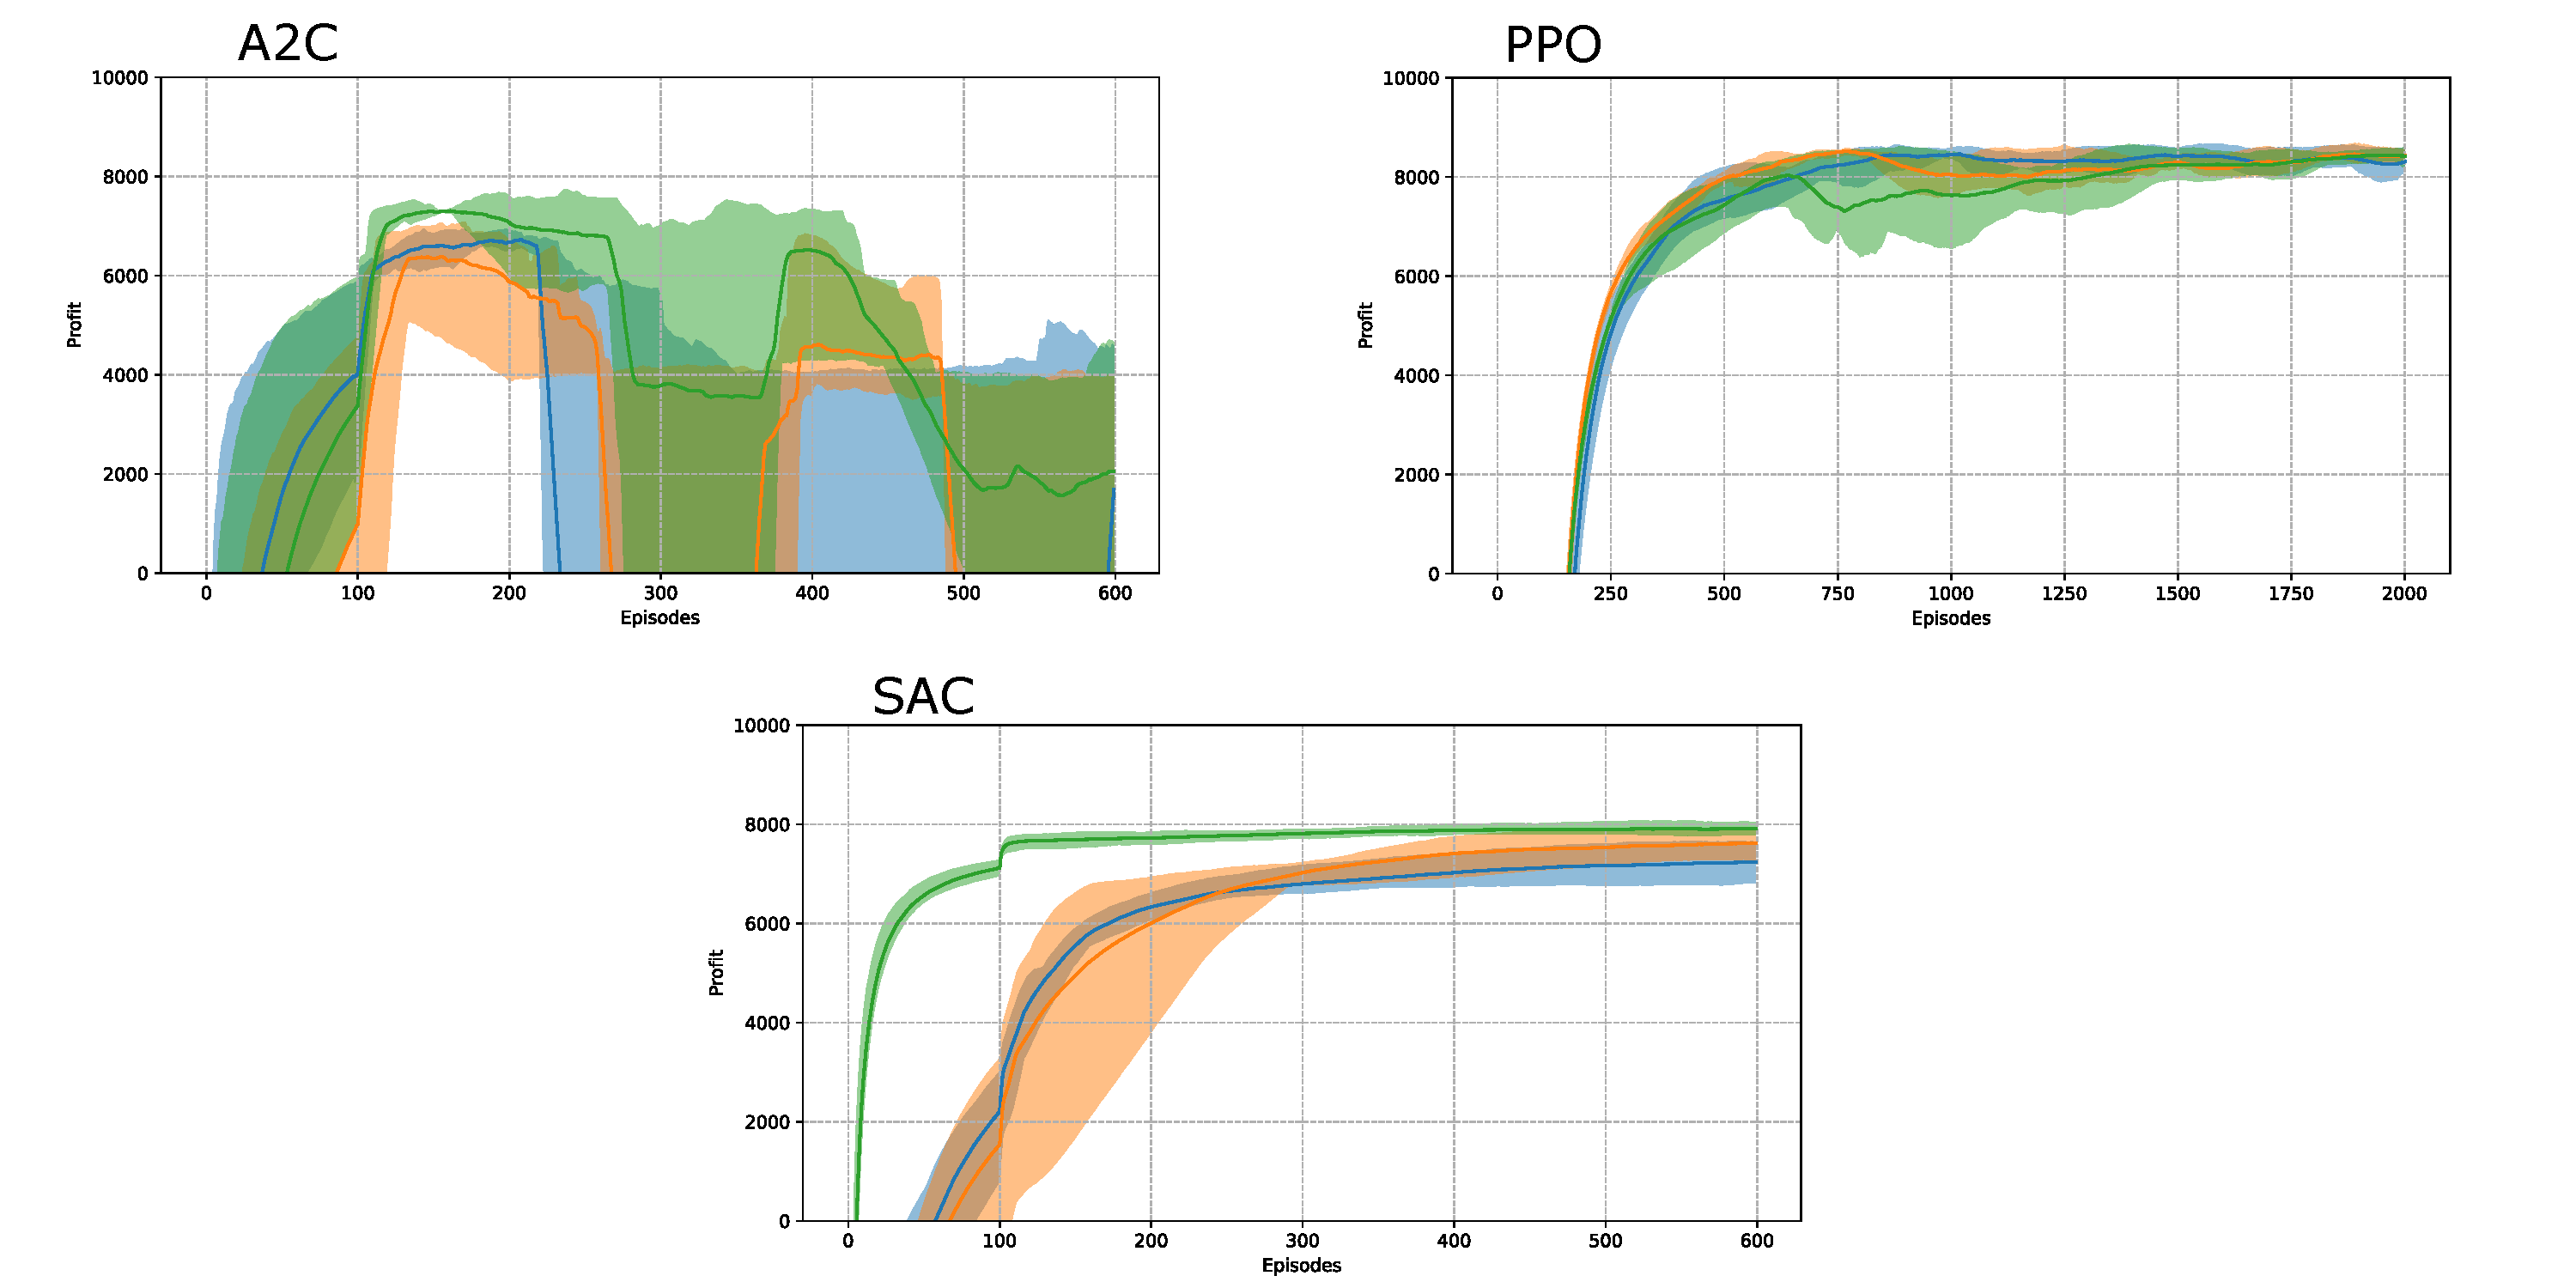
\includegraphics[width=\textwidth]{main/partial_observation.pdf}
	\caption{Lernkurven von A2C, PPO und SAC bei vollständiger im Vergleich zu partieller Beobachtung; (blau) vollständige Beobachtung, (orange) ohne Lagerstand des Konkurrenten und (grün) ohne Lagerstand des Konkurrenten und Anzahl der Produkte
	}
	\label{graphic:PartialObservation}
\end{figure}

In Abbildung \ref{graphic:PartialObservation} sind die Lernkurven der drei Algorithmen beim Training gegen die unterbietende, regelbasierte Strategie dargestellt.
Das Ergebnis fällt dabei äußerst überraschend aus.
Die Erwartung, dass weniger Informationen zu schlechteren Ergebnissen führen müssten, erfüllt sich nicht.
Bis auf eine leicht verschlechterte Stabilität ist die Performance bei PPO ähnlich.
Dieses geringfügige Absinken der Stabilität lässt sich vermutlich direkt durch das Fehlen von Informationen erklären.
Bei A2C verbessert sich ohne diese Informationen die Performance, und bei SAC sogar deutlich.
Während die SAC-Agenten, denen nur der Lagerstand des Konkurrenten vorenthalten wird, recht ähnliche, leicht verbesserte Ergebnisse wie die mit vollständiger Information erzielen, sind die Agenten, bei denen zusätzlich die Information über die Anzahl der Produkte in Zirkulation fehlt, deutlich besser.
Es senkt sich nicht nur die Zeit bis zum Erreichen der Leistungsspitze auf unter 100 Episoden, sondern es verbessert sich sogar die endgültige Performance.
Damit reicht die Leistung näher, aber nicht ganz an die von PPO heran.
Das ist eine wichtige Erkenntnis mit Blick auf die praktische Anwendbarkeit, und dennoch stellt sich die Frage, wie sich die unerwartet gute Leistung mit unvollständiger Information erklären lässt.

Zur Erklärung ist zunächst heranzuführen, dass die ausgelassenen Informationen nur eine nachgeordnete Rolle spielen.
Sie erklären zwar zu einem Teil die künftige Aktion des Konkurrenten und die Anzahl der verkaufswilligen Eigentümer, allerdings sind die Auswirkungen so indirekt, dass sie schwer für die Verbesserung einer Policy zu verwerten sind. \footnote{Die regelbasierten Konkurrenten verwenden diese Information auch nicht.}
Ein höherdimensionaler Beobachtungsraum stellt zudem grundsätzlich für Machine-Learning-Verfahren eine Herausforderung dar.
Es steigt dann der Bedarf an Samples, Muster in den Daten sind schwerer zu erkennen.

\begin{figure}[htb]
	\centering
	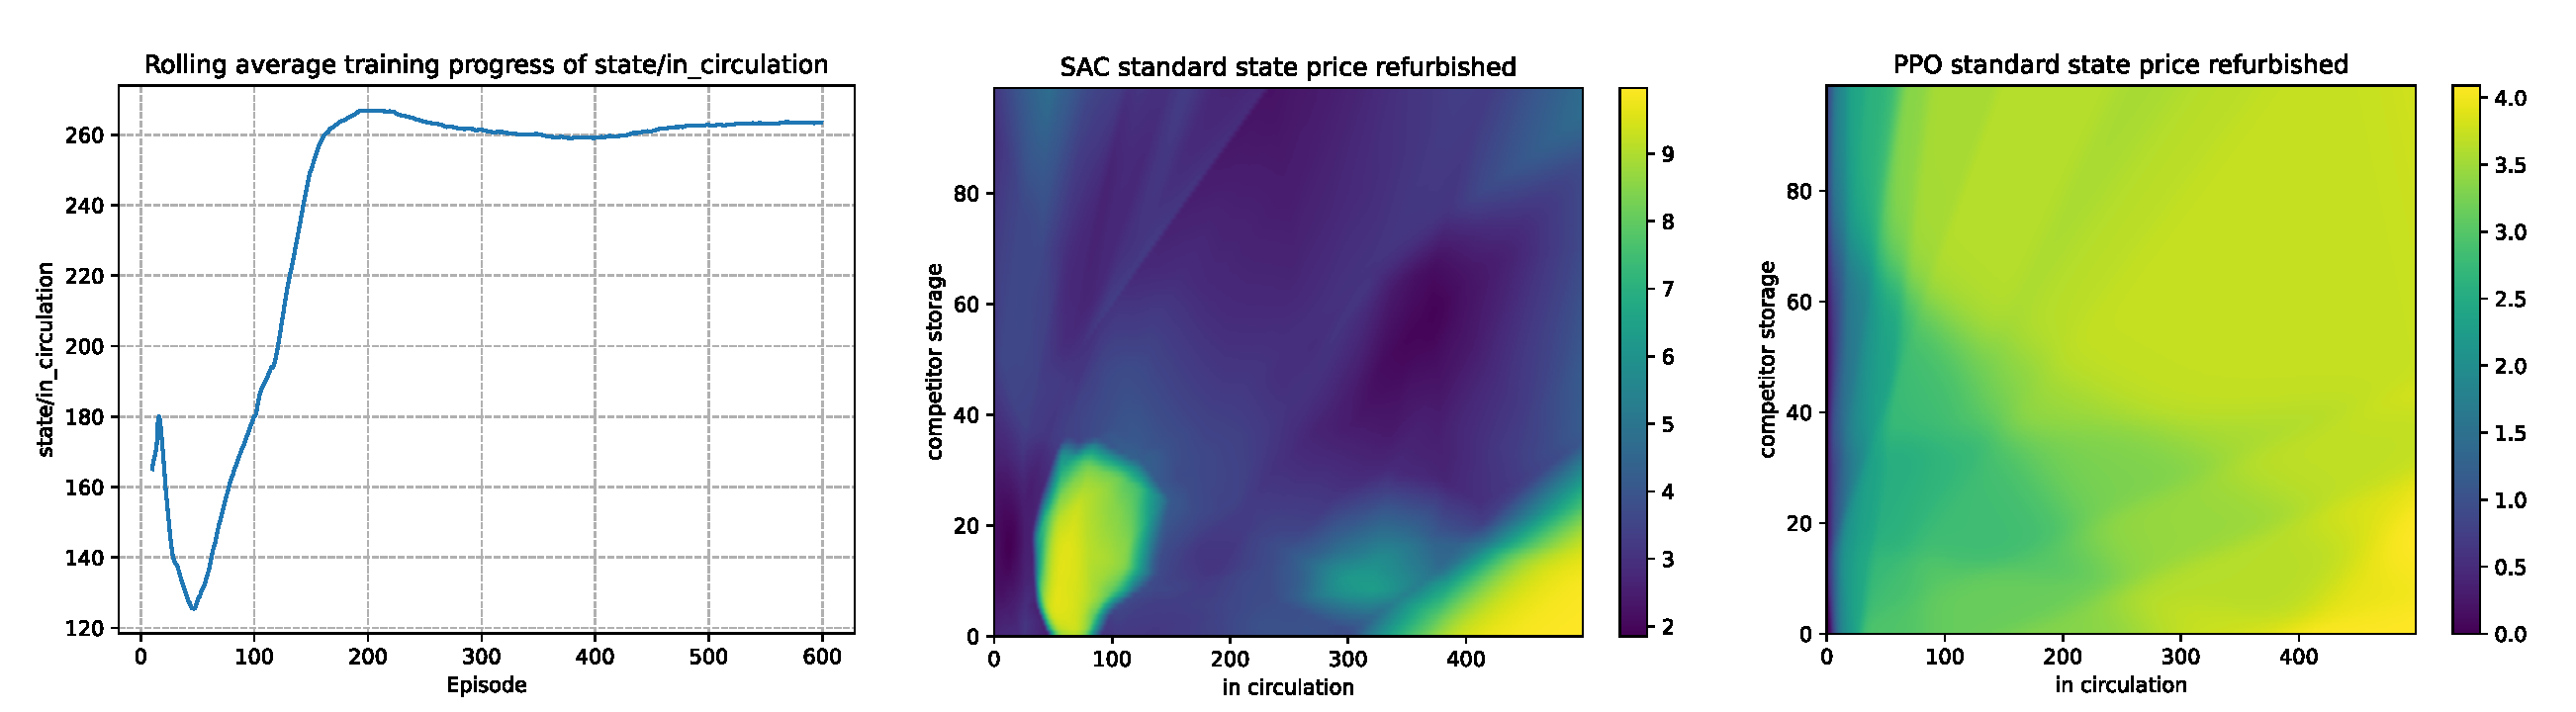
\includegraphics[width=\textwidth]{main/sac_in_circulation_dependend_explanation.pdf}
	\caption{Betrachtung der Agenten mit vollständiger Information: (links) Verlauf des \textit{in-circulation}-Zählers im SAC-Training, (mittig und rechts) Gebrauchtpreis in Abhängigkeit von \textit{in-circulation} und Lagerstand des Konkurrenten bei SAC und PPO; andere Argumente sind dabei fest auf einen Wert gewählt, der typisch bei einem Trainingsdurchlauf ist (eigener Lagerstand: 25, Neupreis Konkurrent: 6, Gebrauchtpreis Konkurrent: 4, Rückkaufpreis Konkurrent: 0)}
	\label{graphic:InCirculationExplain}
\end{figure}
Für die Erklärung des speziellen Phänomens bei SAC genügt die höhere Dimension allerdings nicht.
Ein weiterer Erklärungsansatz drängt sich auf.
Zunächst kann aus Abbildung \ref{graphic:InCirculationExplain} (Mitte) gelesen werden, dass ein SAC-Agent starke Abhängigkeiten von den beiden Argumenten (Zähler der Anzahl in Zirkulation und Lagerstand des Konkurrenten) erlernt.
So unterscheidet sich der Mittelwert der SAC-Policy für Gebrauchtpreise bei ähnlichen Situationen zwischen 2 und 10, ein Sprung durch den gesamten Aktionsraum.
Dass sich eine nahezu optimale Policy so verhalten sollte, ist angesichts der geringen Bedeutung der beiden Argumente auszuschließen, was die Policy des deutlich erfolgreicheren PPO-Agenten bestätigt.
Wie man es erwarten würde, hängt sie kaum von diesen beiden Argumenten ab.
Die niedrigeren Leistungsmaxima von SAC lassen sich vermutlich durch derartige Schwächen der Policy erklären.

Für die von SAC erlernte Policy lässt sich eine Erklärung in der Funktionsweise von Soft Actor Critic finden.
Sie basiert darauf, dass bei weiterentwickelten Policies im Markt mehr Produkte in Zirkulation sind.
Das ist in Abbildung \ref{graphic:InCirculationExplain} (links) gezeigt und liegt daran, dass wenig trainierte Policies im Gegensatz zu den weiterentwickelten oft zu viel zurückkaufen (und dabei zu viel Geld ausgeben).
Das bedeutet, dass gerade am Anfang der Experiencebuffer nur mit Zustandsübergängen mit niedrigen \textit{in-circulation}-Werten gefüllt wird.
Diese Samples bleiben im Experiencebuffer, sind aber für das spätere Training nicht mehr hilfreich und können die Anomalien in der Policy erklären.
So liegt eine starke Anomalie in der Policy im Bereich zwischen 50 und 150 Produkten in Zirkulation, genau der Bereich, aus dem die frühen Samples stammen.
Das Entfallen des \textit{in-circulation}-Eintrages verbessert also die Performance des SAC wohl deshalb, weil dieser dann nicht mehr die Möglichkeit hat, mit missweisenden Samples tatsächlich nicht existente Zusammenhänge zu erlernen.
Es ist damit als Schwäche von SAC gegenüber dem On-Policy-Verfahren PPO zu verzeichnen, dass es weniger gut in der Lage ist, die geringe Relevanz dieses Attributes selbstständig zu erlernen.

\section{Durch die Policy induziertes Marktgeschehen}
Die vorigen Untersuchungen bewerteten die Leistung der Policy vorrangig anhand der Leistung, die ein Agent über den Trainingsverlauf hinweg erzielt.
Es lohnt sich jedoch ebenfalls, eine einzelne Episode genauer zu betrachten.
Dabei interessiert man sich dafür, ob situationsangemessene Preise gewählt werden, ob das Lager erfolgreich reguliert wird und ob sich Gleichgewichte einstellen.
Es muss jedoch beachtet werden, dass es sich um exemplarische Durchläufe handelt.
Bei Verallgemeinerungen ist deshalb große Vorsicht geboten.

Im ersten Durchlauf einer Episode wurde ein PPO-Agent gegen den unterbietenden regelbasierten Wettbewerber getestet.
Es handelt sich bei dem PPO-Agenten um die Modellparameter, die bei dem Self-Play-Durchlauf mit gemischter Belohnungsfunktion trainiert wurden, dessen Trainingsverlauf in \mbox{Abbildung \ref{graphic:SelfPlayDetails}} abgedruckt wurde.
Details aus dieser Episode sind im Anhang in Abbildung \ref{graphic:EpisodeAnalysisPPOvsRulebased} abgedruckt.
Dabei wurden die Lagerstände der beiden Agenten über die vollen 500 Schritte der Episode abgedruckt.
Von den gesetzten Preisen wurde ein 25-Schritte-Intervall zum Ende der Episode gezeigt.
Zunächst ist zu erkennen, dass beide Agenten einen Startzustand mit unerwünscht hohem Lagerstand bekommen.
Bei PPO ist die Initialisierung fast beim Maximum.
Beide Agenten leeren nun ihre Lager, um Lagerkosten zu sparen.
Nach weniger als 50 Schritten pendelt sich das Lager bei beiden Agenten um 10 Produkte herum ein.
Während dieser Wert beim regelbasierten Agenten fest einprogrammiert ist, hat sich der PPO-Agent ein sehr ähnliches Niveau beim Training selbst beigebracht.
Die Lagerschwankungen, die sich eingestellt haben, sind beim regelbasierten Agenten kleiner als beim PPO-Agenten.
Eine naheliegende Erklärung dafür ist, dass der regelbasierte Agent den vorgegebenen Lagerstand sehr aggressiv regelt.
So ist bei Rückkauf- und Gebrauchtpreis zu sehen, dass beinahe jeden Schritt zwischen einem sehr niedrigem und einem sehr hohen Preisniveau gewechselt wird.
Die Unterschiede zwischen benachbarten Preisen fallen bei dem RL-Agenten deutlich niedriger aus.
Man kann auf Basis dieser Diagramme vorschlagen, dass der regelbasierte Agent bei der Regulierung des Lagers größere Toleranz walten lassen könnte, um die Preissprünge zwischen aufeinanderfolgenden Schritten zu reduzieren.
Bei den Neupreisen sieht man ebenfalls die einprogrammierte Logik im Preisverlauf:
Der regelbasierte Agent setzt hier keine eigenen Impulse und unterbietet den PPO-Agenten stets um eins.
Dadurch ist seine Kurve die um einen halben Schritt nach rechts und eine Preisstufe nach unten versetzte Kurve des PPO-Agenten.
Am Ende der Episode stehen als Profite 7994 für den PPO-Agenten gegen 5844 des regelbasierten Agenten.

Neben der Gegenüberstellung mit dem regelbasierten Agenten wurde eine Episode des PPO-Agenten gegen einen ebenfalls mit gemischter Rewardfunktion und Self-Play trainierten SAC-Agenten untersucht.
Dabei wurden die gleichen Diagramme erstellt.
Sie sind im Anhang in \mbox{Abbildung \ref{graphic:EpisodeAnalysisPPOvsSAC}} zu finden.
Die Initialisierung geschah wie im obigen Verlauf mit deutlich mehr Produkten im Lager als gewünscht, die dann abverkauft werden, bis sich der Lagerstand beider Agenten unter 20 einpegelt.
Das Preisniveau für Neuprodukte ist bei beiden Agenten auf ähnlichem und stabilen Niveau und bewegt sich zwischen 5 und 6.
Während die anderen Preise sich ebenfalls auf relativ stabilem Niveau bewegen, sticht der Gebrauchtpreis des SAC-Agenten hervor.
Er ist stärkeren Schwankungen zwischen 2 und 9 unterworfen.
Am Ende der Episode liegt der PPO-Agent mit 9920 zu 9319 vor dem SAC-Agenten

\section{Vergleich im Monopol}
In den vorigen Abschnitten wurden die Algorithmen in einem Recommerce-Duopol mit einem regelbasierten, unterbietenden Konkurrenten getestet.
Für reale Anwendungen sind aber viele verschiedene Szenarien zu meistern.
Es ist daher von Interesse, wie die Algorithmen auf verschiedenen Marktszenarien abschneiden, die in der Praxis auftreten können.
Ein Szenario, das leichter ist sein dürfte, ist das Monopol.
Hier ist der RL-Agent der einzige Anbieter, während weiterhin die gleiche Anzahl von Kunden den Markt besucht.
Die anderen Dynamiken des Marktes sind unverändert.
Als Rewardfunktion wird der Gewinn des Agenten gewählt -- Vergleiche mit Konkurrenten erübrigen sich im Monopol.

\begin{figure}[htb]
	\centering
	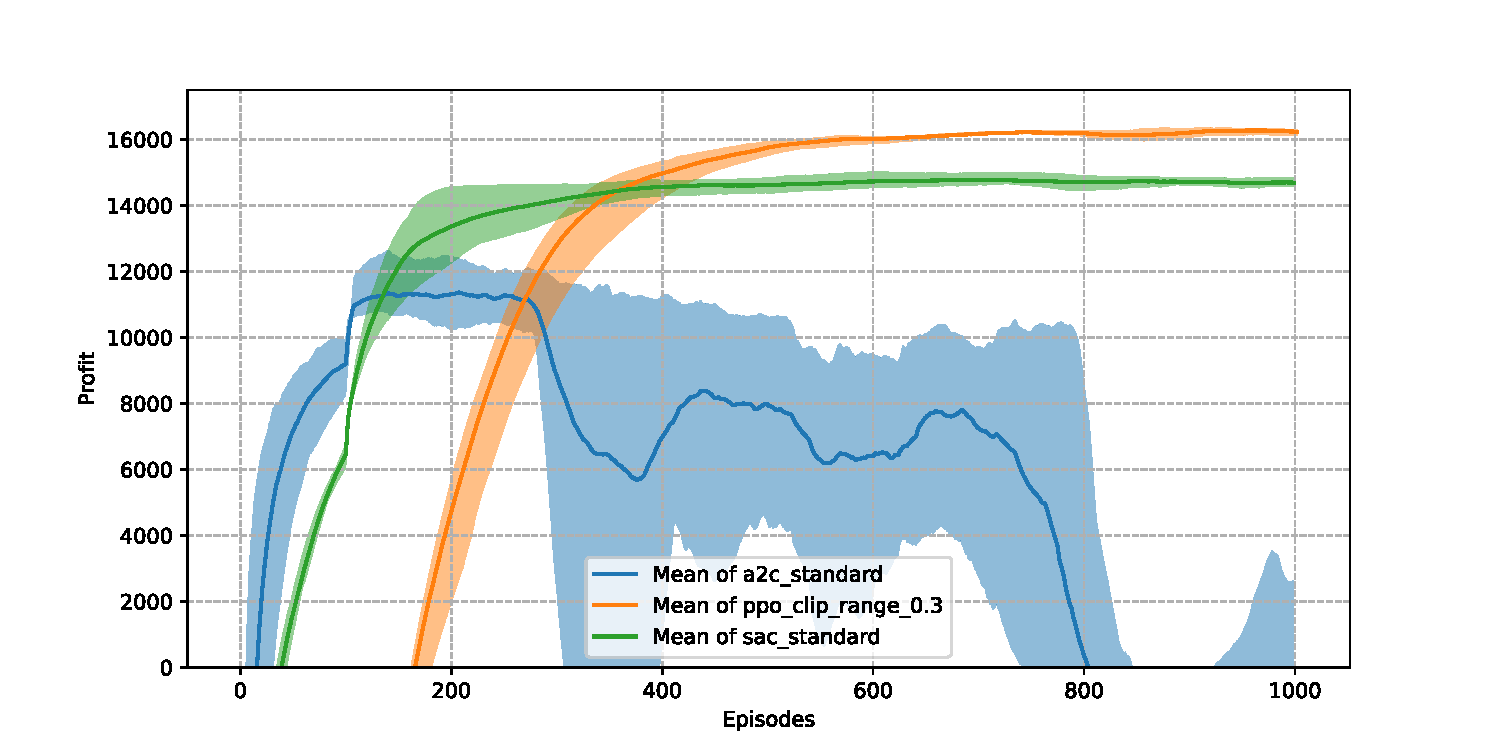
\includegraphics[width=\textwidth]{main/comparison_monopoly.pdf}
	\caption{Lernkurven von vier A2C-, PPO- und SAC-Durchläufen in einem Monopolszenario über 1000 Episoden}
	\label{graphic:MonopolyComparison}
\end{figure}

Abbildung \ref{graphic:MonopolyComparison} zeigt die Lernkurven der drei Agenten auf dem Monopolmarkt mit vollständiger Information.
Dabei stechen sofort die Parallelen zum Duopol-Markt ins Auge:
\begin{enumerate}
	\item Die relative Reihenfolge der Agenten bei der Lernkurve ist die gleiche: PPO schneidet am besten ab, dann SAC vor A2C.
	\item A2C erreicht als erstes die Gewinnzone, danach folgt SAC und zuletzt PPO.
	\item Das Training von PPO und SAC ist sehr stabil, A2C-Training ist von Abstürzen geprägt.
\end{enumerate}
Auch wenn der Monopol-Markt einfacher ist, so benötigt das Training nicht erheblich weniger Samples.
Vergleicht man den Punkt, an dem die Algorithmen keine deutlich besseren Ergebnisse mehr erreichen, liegt A2C in beiden Setups bei 100 bis 200 Episoden, SAC bei etwa 300 Episoden und PPO bei etwa 600 Episoden.

Im Monopol erzielen diese drei Algorithmen etwa doppelt so hohe Gewinne wie im Duopol.
Auf der einen Seite ist das plausibel, schließlich müssen sie sich den Markt nicht mehr aufteilen.
Auf der anderen Seite könnte man aber erwarten, dass die Gewinne sogar höher ausfallen, indem die Monopolsituation durch Verlangen höherer Preise ausgenutzt wird.
Dass dies nicht geschieht, liegt an der begrenzten Kaufbereitschaft der Kunden, gerade bei höheren Preisen.
Im Anhang in Abbildung \ref{graphic:PPOMonopolyDuopoly} wird dazu ein PPO-Durchlauf im Monopol mit einem im Duopol mit Blick auf Verkaufszahlen verglichen.

\section{Vergleich im Oligopol}
Als weiteres Szenario wird das Oligopol untersucht.
Dabei tritt der RL-Agent gegen die folgenden Agenten an:
\begin{enumerate}
	\item eine Verallgemeinerung des bekannten regelbasierten Agenten (unterbietet das Minimum der anderen um eins),
	\item einen regelbasierten Agenten, der mithilfe der Preise zwar sein Lager reguliert, aber nicht auf die anderen Agenten reagiert,
	\item einen Agenten, der feste Preise hat (6 als Neupreis, 3 als Gebrauchtpreis und 2 als Rückkaufpreis) und
	\item einen Agenten, der speziell für das Oligopolszenario erstellt wurde.
	Als Neupreis unterbietet er den Median der anderen Anbieter, und reguliert sein Lager so, dass es etwa 7 Produkte enthält.
\end{enumerate}
Jeder Schritt wird hier in Fünftel zerlegt, die Anbieter setzen ihre Preise reihum.
In jedem dieser Fünftel kommen vier Kunden zum Marktplatz, insgesamt also weiterhin 20.
Das sonstige Verhalten des Marktes bleibt unverändert.
Der Beobachtungsraum ist 18-dimensional (\textit{in-circulation}, eigener Lagerstand und für jeden der vier Konkurrenten drei Preise sowie der Lagerstand).
Damit handelt es sich um das komplexeste Szenario, das untersucht wurde.

\begin{figure}[htb]
	\centering
	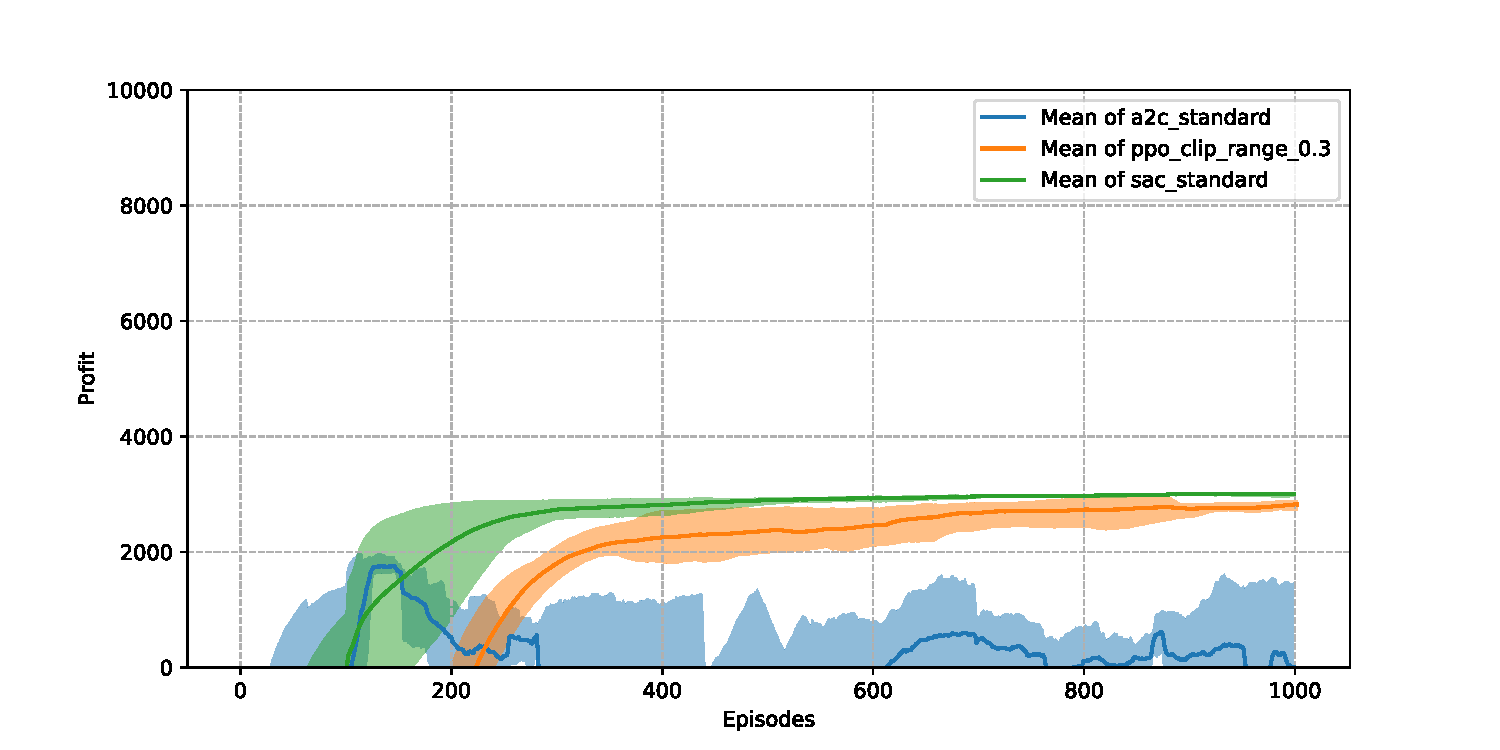
\includegraphics[width=\textwidth]{main/comparison_oligopoly.pdf}
	\caption{Lernkurven von vier A2C-, PPO- und SAC-Durchläufen in einem Oligopolszenario über 1000 Episoden mit normaler Rewardfunktion und vollständiger Beobachtung}
	\label{graphic:OligopolyComparison}
\end{figure}

Grafik \ref{graphic:OligopolyComparison} zeigt die Lernkurven auf diesem Oligopolszenario.
Die RL-Agenten erreichen auch hier Lernerfolg, wobei die Gewinne selbstverständlich niedriger ausfallen, da sich die gleiche Anzahl von Kunden auf deutlich mehr Anbieter verteilt.
Wie auch in den anderen Experimenten, zeigen PPO und SAC stabile Lernkurven.
Bei A2C zeigen sich die bekannten Instabilitäten, aber ihre Leistung in der Spitze bleibt tatsächlich nur leicht hinter der der anderen Algorithmen zurück.
Äußerst interessant ist bei diesem Versuch, dass der SAC-Algorithmus besser abschneidet als PPO, der bei den anderen Experimenten in der Spitzenleistung überlegen war.
Weil wegen des hohen Trainingsaufwandes nur 1000 Episoden trainiert wurden und die PPO-Kurven am Ende noch einen leichten Anstieg zeigen, kann zwar nicht ausgeschlossen werden, dass PPO zu einem späteren Zeitpunkt aufholt, aber dennoch lässt sich auf Grundlage dieser Lernkurve SAC als überlegen einordnen.

Der mutmaßliche Grund hierfür ist das größere neuronale Netz, mit dem SAC arbeitet.
Mit 256 Neuronen in den beiden versteckten Schichten lassen sich kompliziertere Funktionen erlernen als mit nur 64 Neuronen in den versteckten Schichten.
Gerade bei der hier erforderlichen deutlich hochdimensionaleren Policyfunktion ist die Notwendigkeit für eine komplizierte Funktion gegeben.
Um diese Vermutung nachzuprüfen, wurde ein zusätzliches Experiment durchgeführt, bei dem PPO Netze mit 256 Neuronen in den versteckten Schichten trainiert.
Die Lernkurven sind im Anhang in Abbildung \ref{graphic:OligopolyMixedComparisonBigNetwork} abgedruckt.
Dabei zeigt sich, dass gute PPO-Durchläufe schließlich die gleiche Performance erreichen wie bei SAC, aber die Trainingsstabilität erheblich niedriger ist.

Der Algorithmenvergleich auf dem Oligopol wurde ebenfalls mit der gemischten Rewardfunktion durchgeführt.
Dessen Ergebnisse sind ähnlich, allerdings streuen die SAC-Durchläufe dort deutlich stärker.
Die Lernkurven dazu sind im Anhang in Abbildung \ref{graphic:OligopolyMixedComparison} abgedruckt.

\begin{figure}[htb]
	\centering
	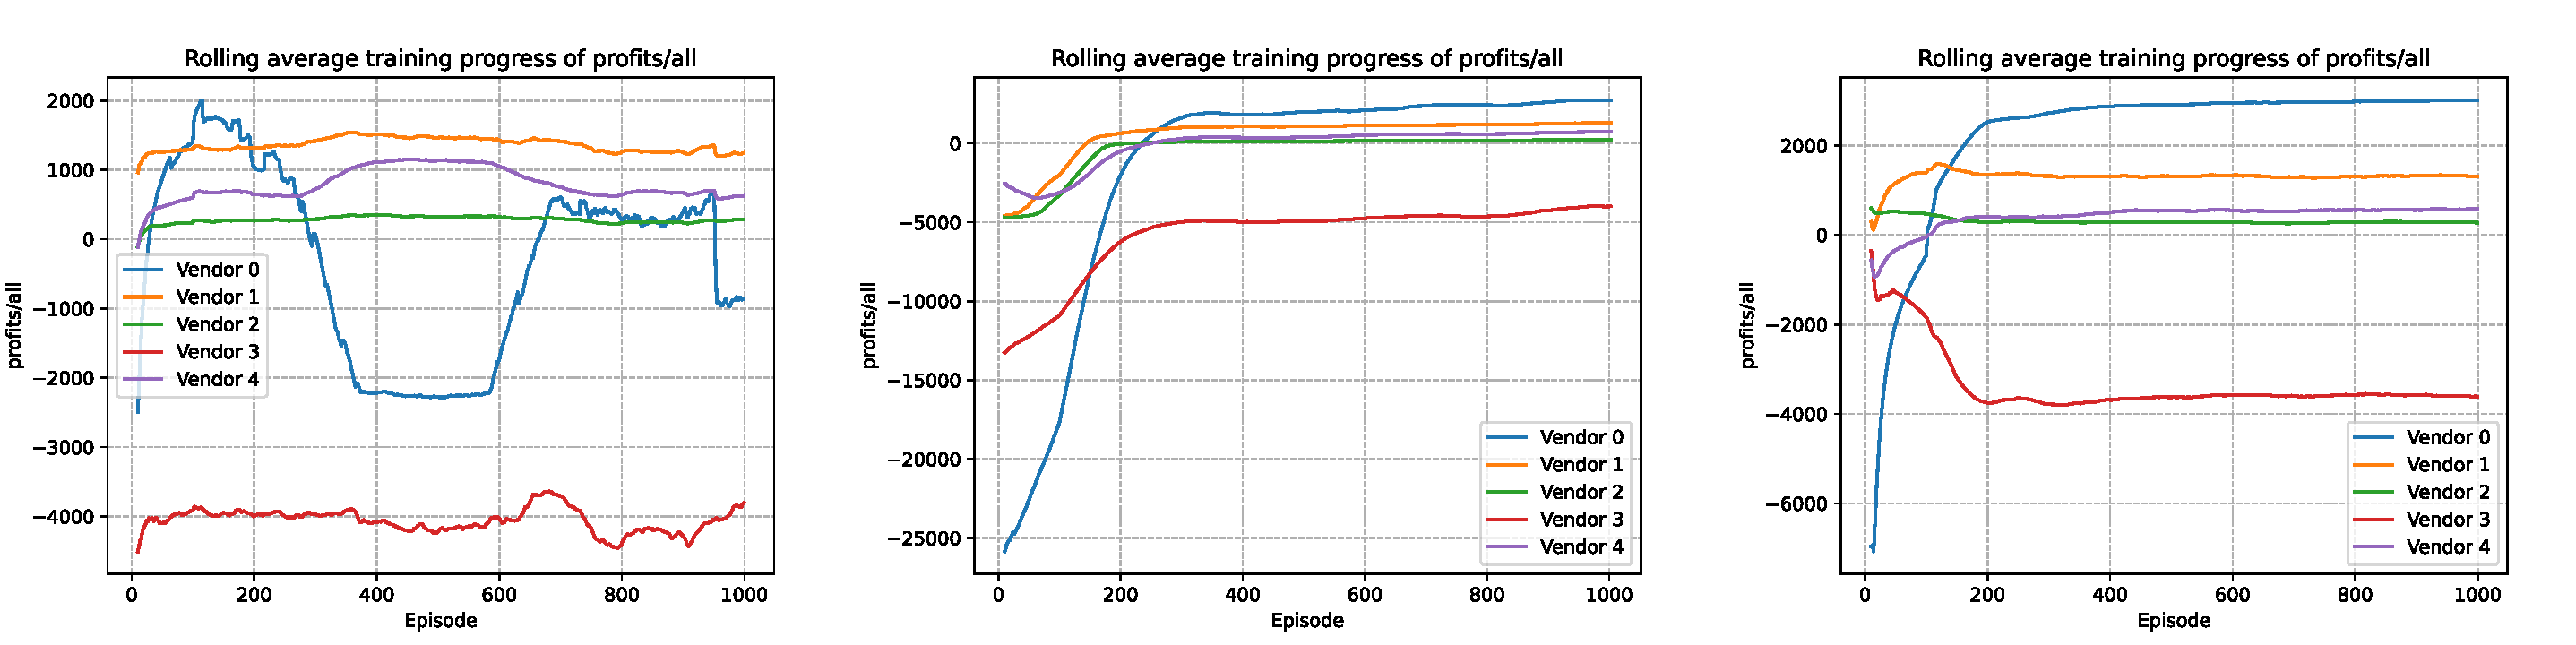
\includegraphics[width=\textwidth]{main/oligopoly_vendor_comparison.pdf}
	\caption{Profite typischer Trainingsdurchläufe von A2C, PPO und SAC im Vergleich zu ihren regelbasierten Konkurrenten}
	\label{graphic:OligopolyVendorComparison}
\end{figure}

Abbildung \ref{graphic:OligopolyVendorComparison} zeigt für jeden der drei Algorithmen einen typischen Trainingsdurchlauf.
Die Ergebnisse sind dabei äußerst zufriedenstellend.
Jeder der RL-Agenten kann während seines Trainingsdurchlaufes alle seine regelbasierten Konkurrenten deutlich übertreffen.
Der Agent mit den festen Preisen schneidet erwartungsgemäß am schlechtesten ab, da er weder dazu in der Lage ist, sein Lager zu regulieren, noch auf Preise der Konkurrenten zu reagieren.
Der Agent, der nur sein Lager reguliert, landet auf dem vorletzten Platz, während die beiden regelbasierten Agenten, die auch auf Konkurrenzpreise reagieren, passabel abschneiden.

In diesem Oligopolszenario tritt der Effekt, dass ein RL-Agent einen regelbasierten Konkurrenten überholen lässt, nicht auf.
Weil die RL-Agenten ihre Konkurrenz hier stets überholen, besteht nicht die Notwendigkeit für die gemischte Rewardfunktion.
Deshalb werden diese Versuche auch nicht detailliert betrachtet.